\documentclass[oneside,12pt]{discsthesis}
\usepackage{graphicx}
\usepackage{multirow}
\usepackage{fancyvrb}
\usepackage{tabularx}
\usepackage[titletoc]{appendix} 
\usepackage{subcaption}
\usepackage{amsmath}
%\usepackage{rotating}
%\usepackage{pdfpages}
\usepackage{lscape}
\usepackage{adjustbox}
\usepackage{longtable}
\usepackage{url}

\title{FinalManuscript_DISCS_UG}
\author{acalab.imagegroup }
\date{March 1, 2018}

\begin{document}

\ThesisAuthor{\textbf{Joshua Roland B. Cruz}}
\ThesisTitle{TESTING A DIFFERENT TITLE}
\ThesisArea{Computer Science}
\ThesisDefenseYear{2019}
\DefenseDate{2018}
%\ThesisGrade{Excellent}
 
\DepartmentHead{ANDREI D. CORONEL, Ph.D.}
\SchoolHead{RAPHAEL A. GUERRERO, Ph.D.}
\ThesisAdviser{MA. REGINA JUSTINA E. ESTUAR, Ph.D.}
\FirstPanelMember{PATRICIA ANGELA R. ABU, Ph.D.}
\SecondPanelMember{MARLENE M. DE LEON, Ph.D.}
\ThirdPanelMember{ANDREI D. CORONEL, Ph.D.}

\ThesisStyle{MS}{Final}{-10pt}{15pt}
  
%% Choices for the 1st argument: MS, PhD
%% Choices for the 2nd argument: Final, FinalWithCorner, Draft

%%\FrontMatter
%\input{acknowledgments}
\begin{thesisabstract}
\paragraph{         }
This study builds on the recommendations of previously done studies on semantic based location approximation as previous findings have indicated that further improvements may be made in the usage of this particular geolocation approach. In light of this, this study attempts to develop a more fine-tuned location approximation model for the geolocation of disaster-related tweets. Two semantic analysis based approaches are explored and implemented in this study: a double filter using Latent Dirichlet Allocation and Latent Semantic Analysis, and the usage of Philippine geographic representative dynamic dictionaries in multiple implementations of Latent Semantic Analysis. The accuracy of the geolocated results of both methodologies are measured against the original geolocation information of the queries processed. The results are also visualized to compare the geolocated values against the original values in a clearer manner.
\end{thesisabstract}
\begin{acknowledgments}
We would like to express our deepest gratitude to Dr. Ma. Regina Estuar and Mr. John Noel Victorino, our thesis advisers, for their patience, guidance, and support in the research and implementation of this study. Their willingness to share their knowledge on the subject matter and their efforts in being available for consultations made the completion of this work a reality. 

We would also like to thank Dr. Marlene de Leon and Dr. Andrei Coronel, our thesis panelists, for their constructive and insightful critique that pointed our group to the right direction with regards to our research work. Our work would not be as polished and clear if it weren't for them.

We also wish to acknowledge Mr. Dion Velasco for providing our group with technical resources that helped us test the results of our research work.

Lastly, we wish to thank our families and friends for their undying support and encouragement throughout the development of this work.
\end{acknowledgments}
\tableofcontents
%\listoffigures
%\listoftables

%\MainMatter
%\begin{thesisabstract}
\paragraph{         }
This study builds on the recommendations of previously done studies on semantic based location approximation as previous findings have indicated that further improvements may be made in the usage of this particular geolocation approach. In light of this, this study attempts to develop a more fine-tuned location approximation model for the geolocation of disaster-related tweets. Two semantic analysis based approaches are explored and implemented in this study: a double filter using Latent Dirichlet Allocation and Latent Semantic Analysis, and the usage of Philippine geographic representative dynamic dictionaries in multiple implementations of Latent Semantic Analysis. The accuracy of the geolocated results of both methodologies are measured against the original geolocation information of the queries processed. The results are also visualized to compare the geolocated values against the original values in a clearer manner.
\end{thesisabstract}

\chapter{INTRODUCTION}

The Philippines is considered as one of the most disaster-prone countries in the world. One of the more common disasters that plague the archipelago is typhoons. It is estimated that an average of eight to nine typhoons occur in the area per year \cite{BR2013}.  On top of frequent storms and typhoons, factors such as poor housing and lack of proper response systems have led to heavy losses for the country's citizens \cite{BR2013, WH2014}.  

    Given how the country experiences frequent typhoons, it is important that disaster/typhoon
related information be easily accessible to everyone especially those in the disaster response field. Easy access to accurate and appropriate information will increase the ability of available responders to come up with the most suited type of response to a given scenario. 



\section{Context of Study}

Disaster management systems exist to provide citizens and responders a general, organized approach on how to deal with a certain situation. More systems employ the bottom-up/people-centered approach since a more authority-driven approach has been proven to be insufficient \cite{LEILIUZHANGWANYUEGUO2015, SCOLOBIGPRIORSCHRTERJRINPATT2015}. The bottom-up approach focuses on crowdsourcing, the process of gathering data based on the interactions of users within a certain spectrum.

It is important to note that lack of user participation is problematic since crowdsourcing based management systems heavily rely on data provided by external users. This means that sources of user-provided data that maximize user participation are the optimal sources of information for crowdsourcing based systems. Maximizing   user participation within a platform or network can be achieved by: (1) allowing users to post public content, (2) the existence of a trust management system, and (3) providing users with notifications for events/situations \cite{GOOLSBY2010, VICTORINOESTUARLAGMAY2016}.

Public participation, especially in times of disaster, is vital since information from various angles and contexts provide for a better idea of what is actually happening in different areas. A good source of crowdsourced information nowadays is social media sites. One example is Twitter.

Twitter is a social media networking  site that contains the features that maximize user participation. It is an excellent source of crowdsourced information since it has over a million registered users who can post content and interact with a network of other fellow users. Users may register an account using a smart phone, a tablet or a computer with internet access. Twitter allows its users to create individual profiles, post 280 character-long messages called ‘tweets’, ‘like’, repost or reply to another tweet, and connect with other users by ‘following’ them and vice versa \cite{VIEWEGSTARBIRDPALEN2010}. Content posted by users with public profiles is openly accessible by anyone on the internet. Twitter has been used as a tool to circulate information regarding emergency and disaster related incidents \cite{GOOLSBY2010, VIEWEGSTARBIRDPALEN2010, MCDOUGALL2011} .   Incidents such as the terrorist attacks in Mumbai, India in 2008 and the Queensland floods in Australia in 2011 have shown how social media sites, Twitter in particular, contribute to better disaster risk management and response.

A key component in Twitter that contributes to disaster management is the geolocation information that users may provide. Users provide latitude and longitude coordinates either by indicating a location on their profiles or by turning on their location feature whenever they tweet. Being able to track where a disaster related tweet was sent from gives that tweet more depth as it describes something that is happening at a particular location. The more accurate information on a certain location, the easier it will be for responders to decide how to handle the situation in that location.

However, as large a database of useful information Twitter is, only a small percentage of tweets are geotagged. Previous research found that only around 0.42-1 percent of users allow their tweets to be geotagged \cite{CHENGCAVARLEELEE2010, MAHMUDNICHOLSDREWS2014} and less than 2 percent of total tweets contain location details \cite{LAYLAVIRAJABIFARDKALANTARI2016}. While using Twitter data is effective in disaster management, methods on how to process these data can still be improved.

This opens the door for location approximation for disaster management. Since the majority of tweets are non-geotagged, the need for methods on how to approximate the location of a non-geotagged tweet using geotagged tweets becomes clear. Previous studies have explored different methods of approximating the location of non-geotagged tweets \cite{OBCS2013, GFC2012,carmen,ROSALES2017, VELASCOBERMEJODOMINGO2018}. These previous methods of location approximation include text analysis \cite{ROSALES2017, VELASCOBERMEJODOMINGO2018}, geocoding of user information \cite{OBCS2013, GFC2012, carmen}, and reverse geocoding of geographical coordinates \cite{ROSALES2017, VELASCOBERMEJODOMINGO2018}. Results have shown that there is still room for improvement regarding previously explored location approximation methods--text analysis methods proved to be not completely accurate due to the ungrammatical characteristics of tweets \cite{ROSALES2017, VELASCOBERMEJODOMINGO2018}, geocoding of user information proved to be difficult since users may lie about their "home" location \cite{OBCS2013, GFC2012}, and reverse geocoding of geographical coordinates do not always yield valid map locations.   

Thus, the goal of this study is to derive and test Latent Semantic Analysis based methods aimed towards the fine-tuning of previously used concepts and algorithms. Different applications of existing location approximation methods are being explored in order to determine which direction leads to more accurate geolocation results. Algorithms such as Latent Semantic Analysis and Latent Dirichlet Allocation are being used to test the different methods in this study. The results are to be formatted as a JSON file that can be available for graphical visualization
\section{Research Questions}

 This study seeks to answer the question: What other methods may be explored and added to improve the performance of an existing Latent Semantic Analysis based geolocation algorithm? Furthermore, the following sub-questions are also intended to be answered:

\begin{enumerate}
    \item How may a Latent Semantic Analysis based algorithm implemented in Python be improved or modified to produce more fine-tuned geolocation tags? 
    \subitem How may an LSA based geolocation approach be improved given results of previous LSA based methods involving convex hull weighted center/geometric center computations and region segmentation \cite{ROSALES2017, VELASCOBERMEJODOMINGO2018}?
    \item How will developed models from said implementation/s be visualized and be made available for use by external existing platforms?
    
\end{enumerate}
\section{Research Objectives}
This study aims to test various methods of location approximation for non-geotagged tweets  to determine which approach produces the most accurate geolocation results. The intended results of this study are the following: 

\begin{enumerate}
    \item Derive different variations of Latent Semantic Analysis based methods (e.g. difference in datasets, changes in computing/analysis process)
    \item Test derived Latent Semantic Analysis based methods to compare which variation/s will produce better results relative to results from previous studies.
    \begin{enumerate}[-]
     \item Using different numbers of topics to train semantic models with
     \item Using other semantic models alongside the Latent Semantic Analysis model
    \end{enumerate}
    \item Visualize results of tested methods alongside original dataset values for comparison
\end{enumerate}


\section{Scope and Limitations of the Study}

This study uses mainly the Latent Semantic Analysis algorithm based off previous studies done as mentioned above \cite{ROSALES2017, VELASCOBERMEJODOMINGO2018}. This algorithm is implemented in Python using an extended Python library called Gensim. Algorithms like the Latent Dirichlet Allocation, and tools like the index similarity matrix will also be implemented using the same language and library. 

This study uses a dataset of tweets before and during Typhoon Yolanda collected via Twitter's Streaming API for testing and validation. Tweets containing keywords such as #EarthquakePH, #FloodPH, #WalangPasok, #ReliefPH, and #RescuePH in this time period are considered. 
\section{Significance of the Study}


The significance of this study to the field of computer science is that it contributes to the topic of automated location approximation. The main contribution of this study is related to providing better algorithms for location approximation which is increasingly necessary for geospatial visualization. This study attempts to develop and test methods to produce a more fine-tuned process of the location approximation of tweets. In doing so, it will help future studies on location approximation by providing a point of reference to pick up from. 

The practical significance of this study to the Philippine society is that developing a more accurate way to quickly gather disaster related information will help increase situational awareness among citizens during times of disaster. This will potentially allow responders to obtain accurate information in a short amount of time, which will help them decide on the best course of action to take. 


\chapter{REVIEW OF RELATED LITERATURE}


\section{Twitter and Other Social Media Sites in Disaster Response}
Social media sites provide a vast amount of easily-accessible data for almost anyone who has internet access and a corresponding device. Even during times of disaster, relevant data still circulate across various social media sites. Previous studies have shown that Twitter has been used as a source of data regarding disaster and emergency related matters \cite{GOOLSBY2010, MCDOUGALL2011, VICTORINOESTUARLAGMAY2016, ROSALES2017, VELASCOBERMEJODOMINGO2018}. One particular occasion for instance, is the series of terrorist attacks in Mumbai, India. The terrorist incidents that took place is 2008 resulted in the portrayal of how social media sites may be seen as a source of real-time crisis related information. Twitter users at the time provided authorities with valuable information by tweeting involving situational reports, requests for assistance, and even documentations of the entire series of attacks \cite{GOOLSBY2010}. This instance showed how impactful Twitter may be in times of crisis. Another occasion where social media sites played a key role in during a time of disaster was when a series of tropical cyclones hit Australia. Queensland, a state of Australia, suffered from floods which dramatically affected the lives of local citizens. Major flooding was experienced in over 30 cities, with the cost of damage amounting to billions of dollars. However, this event saw an unprecedented usage of social media sites by the public sector in assisting the local government to keep the situation under control. Local citizens used Twitter and Facebook to post pictures, videos, and status reports that helped members of both the private and public sectors to minimize the damage caused by the flooding \cite{MCDOUGALL2011}. At the peak of the flooding, it was estimated that there were around fourteen to sixteen thousand tweets per hour that contained the ‘qldfloods hashtag’ which was used to facilitate conversations regarding the disaster. Citizens were even applauded by the national government for their contributions via social media sites.

The role of social media sites in disaster risk management continues to grow throughout the years. Aside from the examples discussed above, social media sites have become a potent source of disaster related information that some disaster management systems have already used Twitter as a primary source of data. One example is a Twitter-mining tool called Tweedr which gathers actionable information for responders during and after a disaster \cite{ASHKTORABBROWNNANDICULOTTA2014}. Another is Senseplace2, a web platform that visualizes tweets to increase situational awareness by providing users with geovisual analytics tools to explore the geospatial characteristics of tweets \cite{HSMM2015}. 

\section{Different Types of Disaster-Related Tweets}
There are several different types of tweets that are tweeted by users at different points in time during a disaster \cite{cat2016,TTC2015}. Tweets vary in content and meaning over time since the state of a particular area changes as a disaster progresses. There are tweets that serve as warnings or notices of preparation (pre-disaster tweets such as tweets regarding the name of an upcoming typhoon and possible areas that might be affected), situational reports and rescue requests (during disaster tweets or tweets that concern cries for help and details on the status of a particular sector), and sentiments regarding memorialization (post-disaster tweets which include relief coordination and well-wishes for affected citizens). 

The identification and categorization of disaster-related tweets were analyzed in 2016 \cite{cat2016}. While situational awareness is important for tweet data analysis, it does not fully capture the entirety of the reactions of those who tweet during times of disaster. This study aimed to address that. The study made use of tweets during Hurricane Sandy in the United States back in October 2012. Keyword collection was performed to collect tweets using keywords from October 23, 2012 to April 5, 2013 such as ‘hurricanesandy’, ‘occupysandy’, and ‘sandycam’ to name a few. 

The study used six categories to classify the collected and filtered tweets \cite{cat2016}. The following categories are: Sentiment, Action, Preparation, Reporting, Information, and Movement. Tweets were to be analyzed and classified using annotators and classification models. Two annotators were trained using a segment of tweets in order to design a multi-label schema which annotates tweets that reflect attitudes, information sources, and protective decision-making behavior of those who tweeted. The annotation process involved labeling tweets for relevance, and labeling relevant tweets with their respective categories.

The results of the fine-grained annotations in the study showed that the hardest categories relative to percentage of tweets and k score agreement are Preparation and Movement, while the ones with the most confusions are Preparation, Reporting, and Sentiment. 

\subsection{Methods in Classification}
Support vector machines (SVMs) were the chosen type of classification model for the study as it yielded the best performance measures using feature selection. The baseline features of the study were the counts of unigrams in preprocessed tweets (removal of capitalization, punctuation, and stopwords). Other features such as bigrams, the time of the tweet, whether or not a tweet is a retweet, a tweet’s URL, and word embeddings were also used in the study. 

Classification performance results were computed using the baseline feature (unigrams) only, all the features mentioned, and the best features for each category. It was found that the time, context, and word embeddings features generally help in relevance classification. The most confused categories in terms of classification were Information and Reporting, while the worst performing ones were Movement, Action, and Preparation. The study does discuss that the scores of certain categories were influenced by the sparse dataset they used (e.g. Movement category lacks data). 

Overall, tweets that fall under the categories of Reporting, Information, and Sentiment were the highest in terms of number, annotation score, and classification score despite confusion metrics. In other words, most of the tweets that were collected and analyzed were tweeted during the time of the actual disaster \cite{cat2016}. These were tweets concerned with disseminating first-hand information, spreading news, and expressing emotions, which was also highlighted by the study. Further recommendations of the study dealt with real-time implementation of the methods described onto a real-time, existing platform.

\section{Analysis of Different Types of Tweets During Typhoon Yolanda}
It was mentioned in section 1.5 that this study will be using tweets during Typhoon Yolanda/Haiyan for its purposes. It has been established that there are different types of tweets tweeted at different points in time during a disaster. The case of Typhoon Yolanda is no exception. Citizens in the Philippines and even in other countries used Twitter as a platform to communicate their thoughts and messages when Typhoon Yolanda hit the archipelago \cite{TTC2015}. 

Communication patterns from tweets during Typhoon Yolanda were analyzed in 2015 \cite{TTC2015}. One of the main objectives of the study was to identify the different purposes of the tweets that users from the Philippines tweeted at the time of the disaster. Tweets between November 8, 2013 to November 13, 2013 were collected, a five day span of when the typhoon made landfall in the Philippines. The qualitative software using NVivo was used for data collection. Tweets were collected at three separate time points on each of the five days based on hashtags such as ‘#PrayforthePhilippines’, and ‘#Haiyan’. A random sample of 1000 tweets was then selected for analysis. The majority of the selected tweets were in English, with only a fraction being in the local language Filipino. Only English tweets were analyzed as a result. Over half of the selected tweets were from ordinary citizens, a fifth were from news organizations, and a tenth were from journalists \cite{TTC2015}. 

Analysis was done by first downloading tweets along with metadata such as username, geographic location, and hashtags. Metadata on user geographic location was recoded in order to identify if a tweet was tweeted in the Philippines, outside the Philippines, or unidentified. The selected tweets were then coded, first based on what type of user tweeted a particular tweet (e.g. ordinary citizen, NGO, journalist), and second, based on derived categories of social media use during a disaster. These derived categories are: reporting on the situation from a personal perspective, secondhand reporting, requesting help, coordinating relief efforts, providing mental counseling, criticizing the government, memorializing, discussing causes, and connecting community members.  

Results show that the most common purpose of tweets during Typhoon Yolanda was to report secondhand information. This concerns tweeting about information sourced from other entities such as news reporters, government sites, or testimonies from affected residents. The second most common purpose was memorializing, which concerns expressing sentiments and well-wishes for those affected by the typhoon. The third most common purpose was coordinating relief efforts, tweets that were aimed at organizing relief and rescue operations and calls for donations. This shows that most of the analyzed tweets were tweeted during the time of the actual disaster.

The study also touched on how different types of users used Twitter during the disaster \cite{TTC2015}. It was observed that news organizations, journalists, and government bodies used Twitter mainly for secondhand reporting, while ordinary citizens and celebrities used Twitter for memorializing, and NGOs used Twitter for relief coordination. The relationship between time and Twitter usage was considered as well. Volumes of certain types of tweets changed as Typhoon Yolanda progressed. Number of tweets concerned with secondhand reporting and memorializing were high in number during the first few days of the disaster, but gradually decreased as time passed. On the other hand, the number of tweets concerned with relief coordination was low in volume at first but increased after the storm hit, which indicates an increase in post-disaster response by members of the community.

Another key observation made in the study is the absence of further potential uses of Twitter \cite{TTC2015}. It appeared that the usage of Twitter during Typhoon Yolanda could still be further organized despite apparent communicational patterns. It was seen that particular entities would only be active in tweeting for a given time period during the typhoon. Users used Twitter for traditional purposes instead of maximizing its non-traditional affordances as a non-traditional media platform. A good example is the case of government bodies; government bodies used Twitter for secondhand reporting, but not sufficiently for relief coordination. In this case Twitter could have been used as a platform for better disaster preparedness given its accessibility as a social media site. Journalists did report secondhand information, but the needs of the public go beyond access to secondhand information in the case of a disaster such as Typhoon Yolanda. Affected citizens also did not use Twitter as much to request for assistance during certain points of the Typhoon. Usage of Twitter during times of disasters may still be further explored as the study alludes to.

\section{Previously Explored Approaches to General Location Approximation }
Location is an important aspect of tweets in the context of disaster risk reduction and response. There are several ways of approximating the location of non-geotagged tweets. The location of geotagged tweets are generally recorded and read in the form of latitude-longitude coordinates. Previous methods on approximating the location of tweets without proper latitude-longitude data have been explored \cite{carmen, GFC2012, OBCS2013,ROSALES2017,VELASCOBERMEJODOMINGO2018}. The following section will briefly discuss some of the more common features and approaches used in the location approximation of tweets. 

\subsection{Using ``Place'' JSON Objects}
There are APIs and programs, such as the Twitter Streaming API, that are used to collect tweets from Twitter. Some tweets return a JSON “Place” object which contains coded information regarding that particular tweet \cite{OBCS2013, GFC2012, carmen}. Information such as the country and city of where the tweet was sent from can be found, as well as geographic coordinates. Some Place types include even finer-grained information like street addresses. Twitter itself already performs geolocation for tweets with Place objects. Place objects may be extracted and filtered using various libraries available online \cite{tweepy}.

\subsection{Latitude/Longitude Coordinates of Tweets}
Some tweets contain geographical information in the form of latitude/longitude coordinates. Twitter users may tag their tweets with latitude/longitude coordinates by enabling the location feature of their devices as they tweet. Tweets with latitude/longitude coordinates available indicate the exact location of where a tweet was tweeted from, but they do not necessarily contain fine-grained information unlike tweets with Place objects \cite{OBCS2013, GFC2012, carmen}. Tweets with geographical coordinates are usually used as references in the location approximation of tweets without latitude/longitude data \cite{ROSALES2017, VELASCOBERMEJODOMINGO2018}. Approaches that involve latitude/longitude data include reverse geocoding (translating coordinates to actual locations like cities or provinces) \cite{carmen}, and convex hull geometrics \cite{ROSALES2017, VELASCOBERMEJODOMINGO2018}.

\subsection{User Profile Information}
Twitter allows users to specify a location in the location text field of their profiles. This location is understood to be where a particular user hails from. Tweets from Twitter users who do not turn on their location services when they tweet but have specified locations in their profiles may still be counted as geolocated tweets. The string value that users provide in their profiles may be geocoded and translated \cite{OBCS2013, GFC2012, carmen}. Existing map APIs can resolve profile location strings to structured locations, possibly in the form of latitude/longitude coordinates. It is important to note that geocoded and translated locations are mostly static, which may be problematic since Twitter users may tweet at different locations from their specified ones. Another potential problem is that users may lie or provide nonsensical text in their profiles, which affects approximation accuracy \cite{L12011, L22014}.

\subsection{Content-Based Geolocation}
Tweet content may be analyzed in order to tag a particular tweet with a given location. Factors such as a user’s dialect, mentions, and references may be used to infer where a particular user is located. This particular approach to location approximation is mainly for tweets from users who do not provide explicit location information. There are various possible implementations regarding this approach. One involves analyzing a tweet for mentions of Places of Interest (POI), or terms that pertain to landmarks that may be traced to certain locations in order to approximate the location of a given non-geotagged tweet \cite{L22014, CHENGCAVARLEELEE2010}.  Another involves the application of the Latent Semantic Analysis algorithm, a method of implementation that builds on the assumption that every defined geographic region contains a unique set of word distributions that may be used to geolocate a tweet based on text tweet content \cite{ROSALES2017, VELASCOBERMEJODOMINGO2018}.

\section {Previous Works on Location Approximation in The Context of Typhoon Yolanda }
This study will be based on previous studies regarding the location approximation of non-geotagged tweets during Typhoon Yolanda. Past works have proposed various solutions on how to locate a non-geotagged tweet by using already geotagged tweets as reference. The following section will discuss two previously conducted and related studies that implemented and tested possible location approximation solutions to geolocating tweets in the context of Typhoon Yolanda.

\subsection{Geolocation Approximations to Disaster Related Tweets}
Numerous methods of location approximation involving tweets during Typhoon Yolanda were proposed and explored in 2017 \cite{ROSALES2017}. The particular study made use of local and international tweets tweeted during typhoon Yolanda (internationally known as Haiyan) that contain certain keywords like ‘ulan’, ‘bagyo’, ‘typhoon’, and ‘#Yolanda’. The coordinates of the path of Typhoon Yolanda were also referenced by the study in its work. This study used the latitude/longitude coordinates of tweets as the main feature for location approximation. The study began with an analysis on the spatio-temporal characteristics of disaster related tweets. This was done by looking at the location of the geotagged tweets, the trajectory of different sets of located tweets, and the location of disaster affected areas at different time segments. Sets of computations regarding the correlation among typhoon trajectory, tweet trajectory, and location of disaster affected areas, the relationship between a given number of tweets and the area covered by these tweets, and others were also included in the study \cite{ROSALES2017}.

Tweet texts were converted to document term matrices and fed to an LDA model to perform topic analysis. This was done in order to determine certain themes within a given collection of words that will help determine the location of a certain group of tweets \cite{ROSALES2017}.

Models for disaster location relative location prediction were created to test the theory that distinct regions regarding disaster related information are not geopolitically defined but are determined based on an area’s relative distance to the typhoon or to the disaster affected area. The developed models were used to predict a tweet’s relative distance to the typhoon or the disaster affected area. Tweet texts within defined distances were mined and tokenized before being transformed into a tf-idf matrix. Groups of tweets were compared in order to determine if a particular group belongs to a certain region by predicting the approximated distance from that of the affected area and the eye of the typhoon \cite{ROSALES2017}.

The study also touched on semantic similarity based location approximation models. The study proposed the theory that semantically similar tweets most likely hail from geographically close locations. This particular model made use of three semantic modeling methods: LSA, doc2vec, and tf-idf. The LSA (Latent Semantic Analysis) algorithm was used to measure the semantic similarity of text corpora. Doc2vec was used to generate vector representations of text documents. TF-IDF matrixes were used to determine the importance of a particular word within a corpus. These three tools were used to determine the most semantically similar tweets to a given untagged tweet. In this portion, the location of a non-geotagged tweet was approximated using the coordinates of the most semantically similar tweets to it. Another model was discussed which used three semantic modeling methods \cite{ROSALES2017}.

The created models in the study yielded a variety of results. For the models regarding disaster location relative location prediction, it was found that models for smaller time segments produce better results. Regarding the measurements involving predicting which region a particular group of tweets approximately belong to, it was found that the result is related to the number of tweets in that distance segment. As for location prediction based on the distance of a non-geotagged tweet from the affected area and the typhoon, it was shown that looking at the distance of the query from the affected area produced significantly higher rates of correct predictions \cite{ROSALES2017}. 

For the first model concerning semantic similarity based location approximation, results indicated that the less tweets used for weighted center computation, the better the results. As for the second semantic similarity based model, results showed that there were no significant differences in measurements among the three semantic models \cite{ROSALES2017}.

The recommendations of this study emphasized how semantic based modeling was still in its initial stages. Rigorous testing and more data analysis were suggested in order to determine if the proposed methods of latitude and longitude approximation are appropriate. The study mentioned how the application of the methods tested onto an actual program/site may be helpful in measuring for the accuracies of each \cite{ROSALES2017}.

\subsection{Implementation of Geolocation Approximation Feature for Disaster Systems}
This section will detail a study that continues the work of the study discussed in section 2.2.1. A full pipeline application consisting of four major components was developed and deployed as a service for public use. The four major components are the Tweet Collection Module, the Approximation API, the Geolocation Module, and the Visualization Module. Tweets collected via Twitter’s Streaming API in the Tweet Collector Module are passed to the Approximation API, which connects the Tweet Collector to the Geolocation Module. The Geolocation Module uses Gensim’s (an extended Python library) LSI implementation as a semantic similarity based approach to location approximation. Latent Semantic Indexing (LSI) is similar to LSA, one of the semantic similarity based algorithms discussed in the section 2.2.1. Finally, results produced by the Geolocation Module are displayed using the Visualization Module \cite{VELASCOBERMEJODOMINGO2018}.

The geolocation features of the application are linked with eBayanihan, an existing web and mobile disaster risk management platform in the Philippines that mainly relies on crowdsourced data. The process of the LSI implementation in this study is similar to that the LSA algorithm implementation in the study in section 2.2.1. This study looked at the top ten semantically similar tweets to the said query will be used to form a convex hull with the weight of a given edge equivalent to the query’s percentage of semantic similarity with that particular tweet. Afterwards, the geometric and weighted centers of the convex hull will be calculated to approximate the location of the non-geotagged tweet \cite{VELASCOBERMEJODOMINGO2018}.

Findings show that for one, the geometric center of the convex hull may be used as a substitute for the weighted center regarding the approximation of the latitude and longitude coordinates of a non-geotagged tweet. However, in terms of overall results, most had high standard deviation values, both using lemmatized and non-lemmatized datasets. Another key observation in the study is that narrowing the location range of tweets helped produce more accurate results (lower standard deviation). Meaning, when the possible range approximated values is segmented for further to for example, per region, then more accurate results would be produced. The developed pipeline became available for use online \cite{VELASCOBERMEJODOMINGO2018}. 

Recommendations of the study emphasized that a possible way to implement the method used to produce more accurate results is to segment the geographical territory of the Philippines according to regions. This follows the study’s findings about how the smaller the location range of the tweets, the more accurate the results become. By segmenting the area into regions, perhaps a more accurate set of results will be produced \cite{VELASCOBERMEJODOMINGO2018}. 


\chapter{METHODOLOGY}

This study aims to derive and test various methods of location approximation based on the LSA algorithm. Two proposed methods in particular will be discussed in the following sections. Each method uses the LSA algorithm as a semantic similarity based location approximation of non-geotagged tweets.  As mentioned in Chapter I, all methods are implemented using Python and its extended library, Gensim. Also, the output values of all these methods will be outputted as a JSON file that will be passed on to an existing API or platform for visualization. 

\section{LDA-LSA Combination}


The first proposed method involves using another algorithm in addition to the LSA algorithm, which is the Latent Dirichlet Allocation algorithm.

\subsection{Logic Behind Combining LDA and LSA}

The Latent Semantic Analysis algorithm analyzes a given document of words and compares that said document to an entire collection of other documents to determine which documents that particular query is most similar to in terms of meaning. LSA takes into account factors such as grammar, word usage, and sentence structure to determine which documents or texts convey the same message. A query is given a similarity score to each document in the collection it is being analyzed against which serves as a measure of how similar the meaning of the query is to the meaning of another given text. 

The Latent Dirichlet Allocation algorithm on the other hand takes an entire collection of documents and generates topics based on the underlying themes that can be found in each document in the collection. LDA generates topics in the form of word clouds. Each word in a particular word cloud has a score which represents the weight of that word to that particular topic. In this way, words that point toward a possible point of interest in analysis are grouped together. 

The first proposed methodology seeks to use these two algorithms in succession to test if doing so would help produce a more fine-tuned location approximation model for disaster-related tweets. LDA is implemented first followed by LSA on the collection of words from the dataset mentioned in section 1.4. This methodology first attempts to identify the possible topics Filipinos tweet about before performing semantic analysis. This means that instead of analyzing a given query against all documents in the collection, it will only be analyzed against the documents that contribute to the topic it is most semantically similar to. This allows a given query to be processed using a set of tweets that pertain to just a single theme instead of a wide variety of possible topics. 

\subsection{LDA Model Creation}

The collection of geotagged tweets is first cleaned by removing stop words and words that occur less than 1 percent of the time in the entire collection. The resulting tokens are then inserted into a dictionary as to make it easier to identify the unique words in the collection. The populated dictionary is transformed to a corpus of words afterwards. Both the populated dictionary and transformed corpus are fed to an LDA model created via Python’s Gensim library. The created LDA model will generate only ten topics (tentative) as opposed to the recommended 100-200 since there are generally only a few topics present during a disaster event. 

\subsection{First LSA Model Creation}

Word clouds are formed from all the topics generated by the LDA model by extracting the top ten contributing words for each topic and storing them in a Python list. This list of word clouds is stored in another dictionary and corpus of its own. Both the dictionary and corpus of the word clouds are fed to an LSA model also created via Python’s Gensim library. Afterwards, the corpus of word clouds is wrapped around the created LSA model and is fed to a similarity matrix in preparation for semantic similarity queries. This first LSA model is used to determine which topic a given non-geotagged query is most semantically similar to.

\subsection{Second LSA Model Creation}

Another LSA model is created which uses the original corpus and dictionary of words containing the tokens for all the geotagged tweets in the dataset. The original corpus of words is wrapped around the model and is fed to an accompanying similarity matrix. This second LSA model is used in retrieving the necessary semantic similarity scores for the geolocation approximation of a given query. After identifying which topic a given non-geotagged query is most semantically similar to, the tweets which contribute to that found topic are extracted along with their semantic similarity scores to a particular non-geotagged query.

\subsection{Location Approximation of Non-Geotagged Queries}

Non-geotagged tweets are accepted as queries, and each query is compared to the first similarity matrix to return the similarity score of said query to all the word clouds. In other words, each non-geotagged tweet will be processed to see which topic it is most semantically similar to. The topic with the highest similarity score to a given query is returned then the original corpus of tokens from the geotagged tweets is searched to see which tweets contain any of the top ten contributing words to the said topic. The given query is then processed to the second LSA model and second similarity matrix to retrieve its semantic similarity score against the tweets that contribute to the retrieved topic. The latitude/longitude coordinates of the top ten most semantically similar tweets to the given query among the extracted geotagged tweets are stored in a list and are used to approximate the location of the corresponding non-geotagged tweet query. This entire process will be done for all the non-geotagged tweets in the dataset. 

\section{Dynamic Dictionary Per Geographic Region}

The second proposed method deals with using a set of dynamic dictionaries as reference when it comes to approximating the location of a non-geotagged tweet. This proposed method involves the usage of up to as many geographic regions as there are in the Philippines.
A dynamic dictionary is used per geographic region, meaning there are 17 different dynamic dictionaries that a non-geotagged tweet is compared with for semantic similarity in order to approximate its location. This approach builds on the findings of the study discussed in section 2.5.2; that narrowing the possible approximated location of a non-geotagged tweet to a certain region or area improves geolocation accuracy \cite{VELASCOBERMEJODOMINGO2018}. This method also operates behind the presupposition that people from a particular region or area has a distinct way of talking/tweeting \cite{ROSALES2017, VELASCOBERMEJODOMINGO2018}.

\subsection{Region Assignment of A Given Geolocated Tweet}

First, the geographic boundaries of each Philippine region are identified in terms of latitude/longitude coordinates. This is done with the help of a shapefile which contains all the geographic regions of the Philippines and stores each as a multi-polygon object. A multi-polygon object contains an array of array of points that define the boundaries of a set of closed figures. The geotagged tweets are processed using a Python library called Geopandas in order to assign each tweet to its corresponding geographic region based on its latitude/longitude coordinates. To accomplish this, the shapefile and the dataset containing the geolocated tweets are first converted to geojson files. The two resulting geojson files are then merged using a Python Geopandas function called 'spatial join' to determine which region (using their latitude/longitude coordinates) a given geolocated tweet belongs in. Performing 'spatial join' returns a list where each element contains the list of indices of the geolocated tweets that belong in that integer-represented region. Collections representative of each region are created to store all the geolocated tweets in their appropriate integer-represented region. 

\subsection{Creating Dynamic Dictionaries For Each Region}

All 17 collections of geotagged tweets for each region are transformed to their own dictionaries and corpuses. All dictionaries and corpuses are fed to a corresponding LSA model representative of each Philippine geographic region. All corpuses are wrapped around their corresponding LSA model and are fed to similarity matrices of their own. Non-geotagged tweets are then accepted as queries. Each query is processed by comparing said non-geotagged tweet to all the available LSA models and similarity matrices. The LSA model, along with its corresponding similarity matrix, that returns the ten highest similarity scores to the query is selected as the approximate region that given query belongs to. That LSA model is extracted, and the given non-geotagged query’s similarity scores with the top ten most semantically similar geolocated tweets to it in the corpus of that corresponding model are retrieved and used to approximate the location of the given query. The dictionaries are updated after a certain number of non-geotagged queries have been processed—perhaps after every 500 tweets. Incoming geolocated tweets and formerly non-geotagged tweets with approximated locations are inserted to their corresponding dictionaries, corpuses, and models. All dictionaries, corpuses, and models are then re-instantiated to reflect the changes in content. This is done to simulate an increasingly rich set of models for potentially more accurate geolocation.

\section{Method of Longitude/Latitude Approximation}

The weighted arithmetic mean formula is used to approximate the weighted center of each convex hull formed for each non-geotagged query for both methodologies. Two computations, one for latitude and one for longitude, will be done. The value of each term is the retrieved coordinate (latitude or longitude), and the weight of the said term is its semantic similarity score with the queried tweet. The sum of all these terms is  divided into the sum of the weights of all terms to retrieve the approximated latitude and longitude of the processed non-geotagged tweet.

The logic behind using the weighted arithmetic mean formula to construct the convex hull in which a particular approximated tweet lies in stems from the same idea as to why the LSA algorithm was used for this study. The weighted arithmetic mean formula allows a given query tweet to be analyzed relative to its semantic similarity scores to a given set of geolocated tweets. The typical way of approximating the center of a given polygon is by getting the average of all its coordinates. That way of measurement is not effective for the aims of this study, as it does not take into account the semantic similarity scores of a particular query tweet against the processed tweets of the dataset. The weighted arithmetic mean formula however, factors in the 'weight' or the degree of influence a particular value has in the approximation of another value. This essentially allows a non-geotagged query's approximated latitude and longitude coordinates to be influenced by geolocated tweets in accordance to the assumption of this study that the more semantically similar a given tweet is to another, the more likely the locations of where both tweets were tweeted by their respective users are closer to each other. The multiplication of the semantic similarity score of a query tweet to a geolocated tweet to the latter's latitude/longitude values reflects this idea in the actual geolocation  process.





%\section{Different Sources of Data}

%The third method is more concerned with the geotagged data more than anything else. This study will initially use mined tweets from Twitter, but this approach will attempt to explore other sources of data such as Facebook and other sites. Users on Facebook also have the capacity to indicate their location with posts, either via making a public post or making a check in. Although it may be more complicated than it seems to mine data from Facebook because of recent legal incidents, it is still another site that can be used as a good source of crowdsourced data. There are also hashtags on Facebook similar to Twitter. Other mining tools will be used for sites like Facebook, but the process will be the same by extracting the located posts, configuring them into a dictionary, then a TF-IDF matrix and an LSA model. In this way, the data from Facebook and other sites will be combined with the data from Twitter for a theoretically more accurate dictionary. 
\chapter{RESULTS AND DISCUSSION}
\section{Method of Measuring Accuracy of Approximated Coordinates}
There were three methods used in the measuring of the accuracy of the approximated latitude and longitude coordinates produced by the discussed methodologies in this study. These three are: 1) looking at the Mean Absolute Error of the approximated coordinates compared to the actual coordinates of the tweets in the dataset, 2) using the Haversine Formula to get the average distance of each approximated coordinate from its actual location, and 3) using the Vincety Formula in place of the Haversine Formula. It is to be noted that the LDA-LSA Double Filter (first methodology) used only half of the dataset as test data while the Dynamic Dictionaries Per Region method (second methodology) used the entire dataset. 

\subsection{Mean Absolute Error}
Python's Scikit-Learn library was used in measuring the Mean Absolute Error of the approximated coordinates versus the actual coordinates for both methodologies. The Mean Absolute Error value is a measure which determines the error of all the given values in a dataset relative to another set. The best possible result for a Mean Absolute Error score is 0 since this indicates that there is no disparity between any of the compared values.

The Mean Absolute Error scores for both methodologies are found in \ref{tab:acc_lit}.

\begin {table*}[h]
\centering
\caption {\textbf{Mean Absolute Error Scores of Methodologies}}
\label{tab:acc_lit} 
\begin{tabular}{ c  c  c  c }
\hline
Methodology	&Latitude  	&Longitude 	&Average \\
Type  &MAE   &MAE   &MAE   \\
   \hline

LDA-LSA  &1.66  &1.07  &1.36  \\
Dynamic Dicts. &2.02   &1.30   &1.66   \\  \hline
\end{tabular}
\end{table*}

\subsection{Haversine Formula}
The Haversine Formula is a trigonometric method of measuring the distance of two coordinates. This way of measurement assumes that the two points being measured against one another belongs in a spherical space. 

The results of applying the Haversine Formula to measure the distance of each approximated coordinate versus its actual coordinates are shown in Table 4.2.

\begin {table*}[h]
\centering
\caption {Haversine Formula Scores of Methodologies}
\label{tab:acc_lit2} 
\begin{tabular}{ c  c  }
\hline
Methodology	&Average Haversine   \\
Type  &Distance (in KM)     \\
   \hline

LDA-LSA  &223.94    \\
Dynamic Dicts. &271.71    \\  \hline
\end{tabular}
\end{table*}

\subsection{Vincenty Formula}
The Vincenty Formula functions in a similar way as the Haversine Formula. The only difference is that the Vincenty Formula is a more widely-used method of computation in GPS devices. In principle, the Vincenty Formula uses the same trigonometric principles of computing the distances between two coordinates in a spherical space.

The results of the Vincenty Formula on the two methodologies is shown in Table 4.3.

\begin {table*}[h]
\centering
\caption {Vincenty Formula Scores of Methodologies}
\label{tab:acc_lit3} 
\begin{tabular}{ c  c  }
\hline
Methodology	&Average Vincenty \\
Type  &Distance (in KM)   \\
   \hline

LDA-LSA  &223.15  \\
Dynamic Dicts. &270.75      \\  \hline
\end{tabular}
\end{table*}

\section{Visualization of Results}
This section tackles the visualization of the results of both methodologies. Geolocated tweets were grouped into clusters for the purpose of visualization. The geolocated tweets from the first methodology were clustered based on topics, while the tweets from the second methodology were clustered based on geographic region. 


\begin{figure}
    \centering
    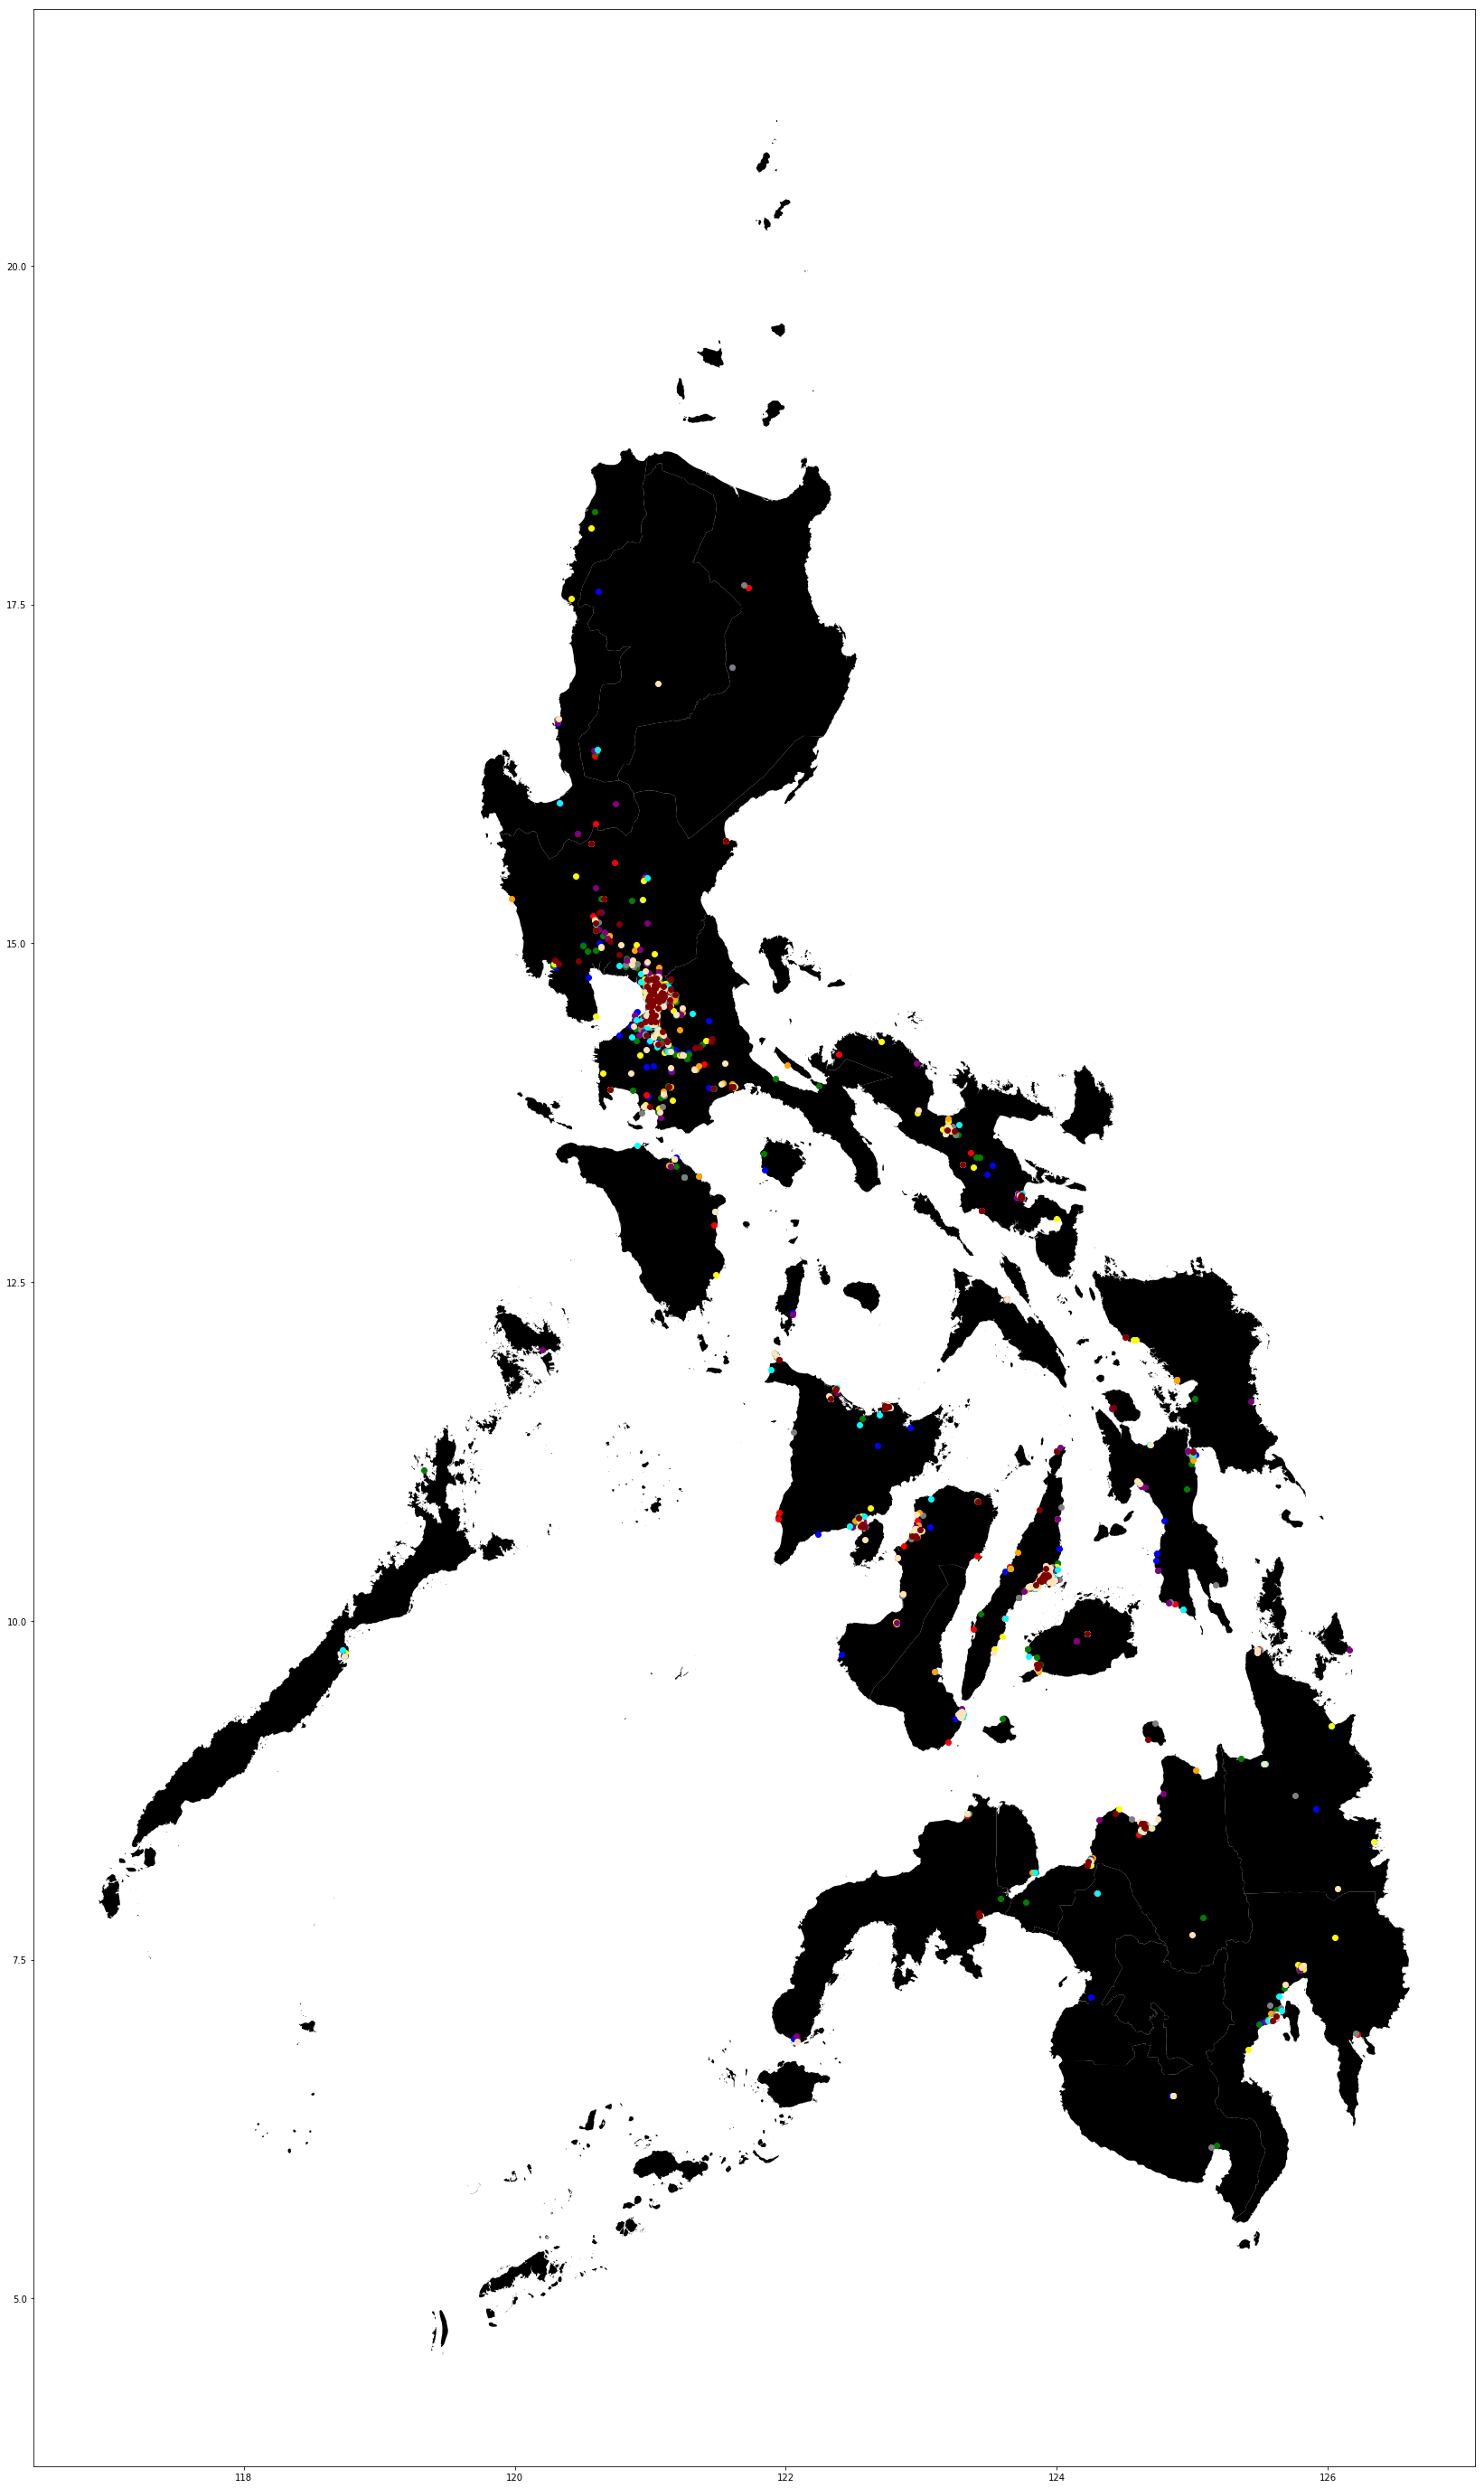
\includegraphics[width=\textwidth, height=\textheight,keepaspectratio]{Method1OrigMap.png}
    \caption{LDA-LSA Double Filter Plot of Original Tweets}
    \label{fig:my_label1}
\end{figure}

\begin{figure}
    \centering
    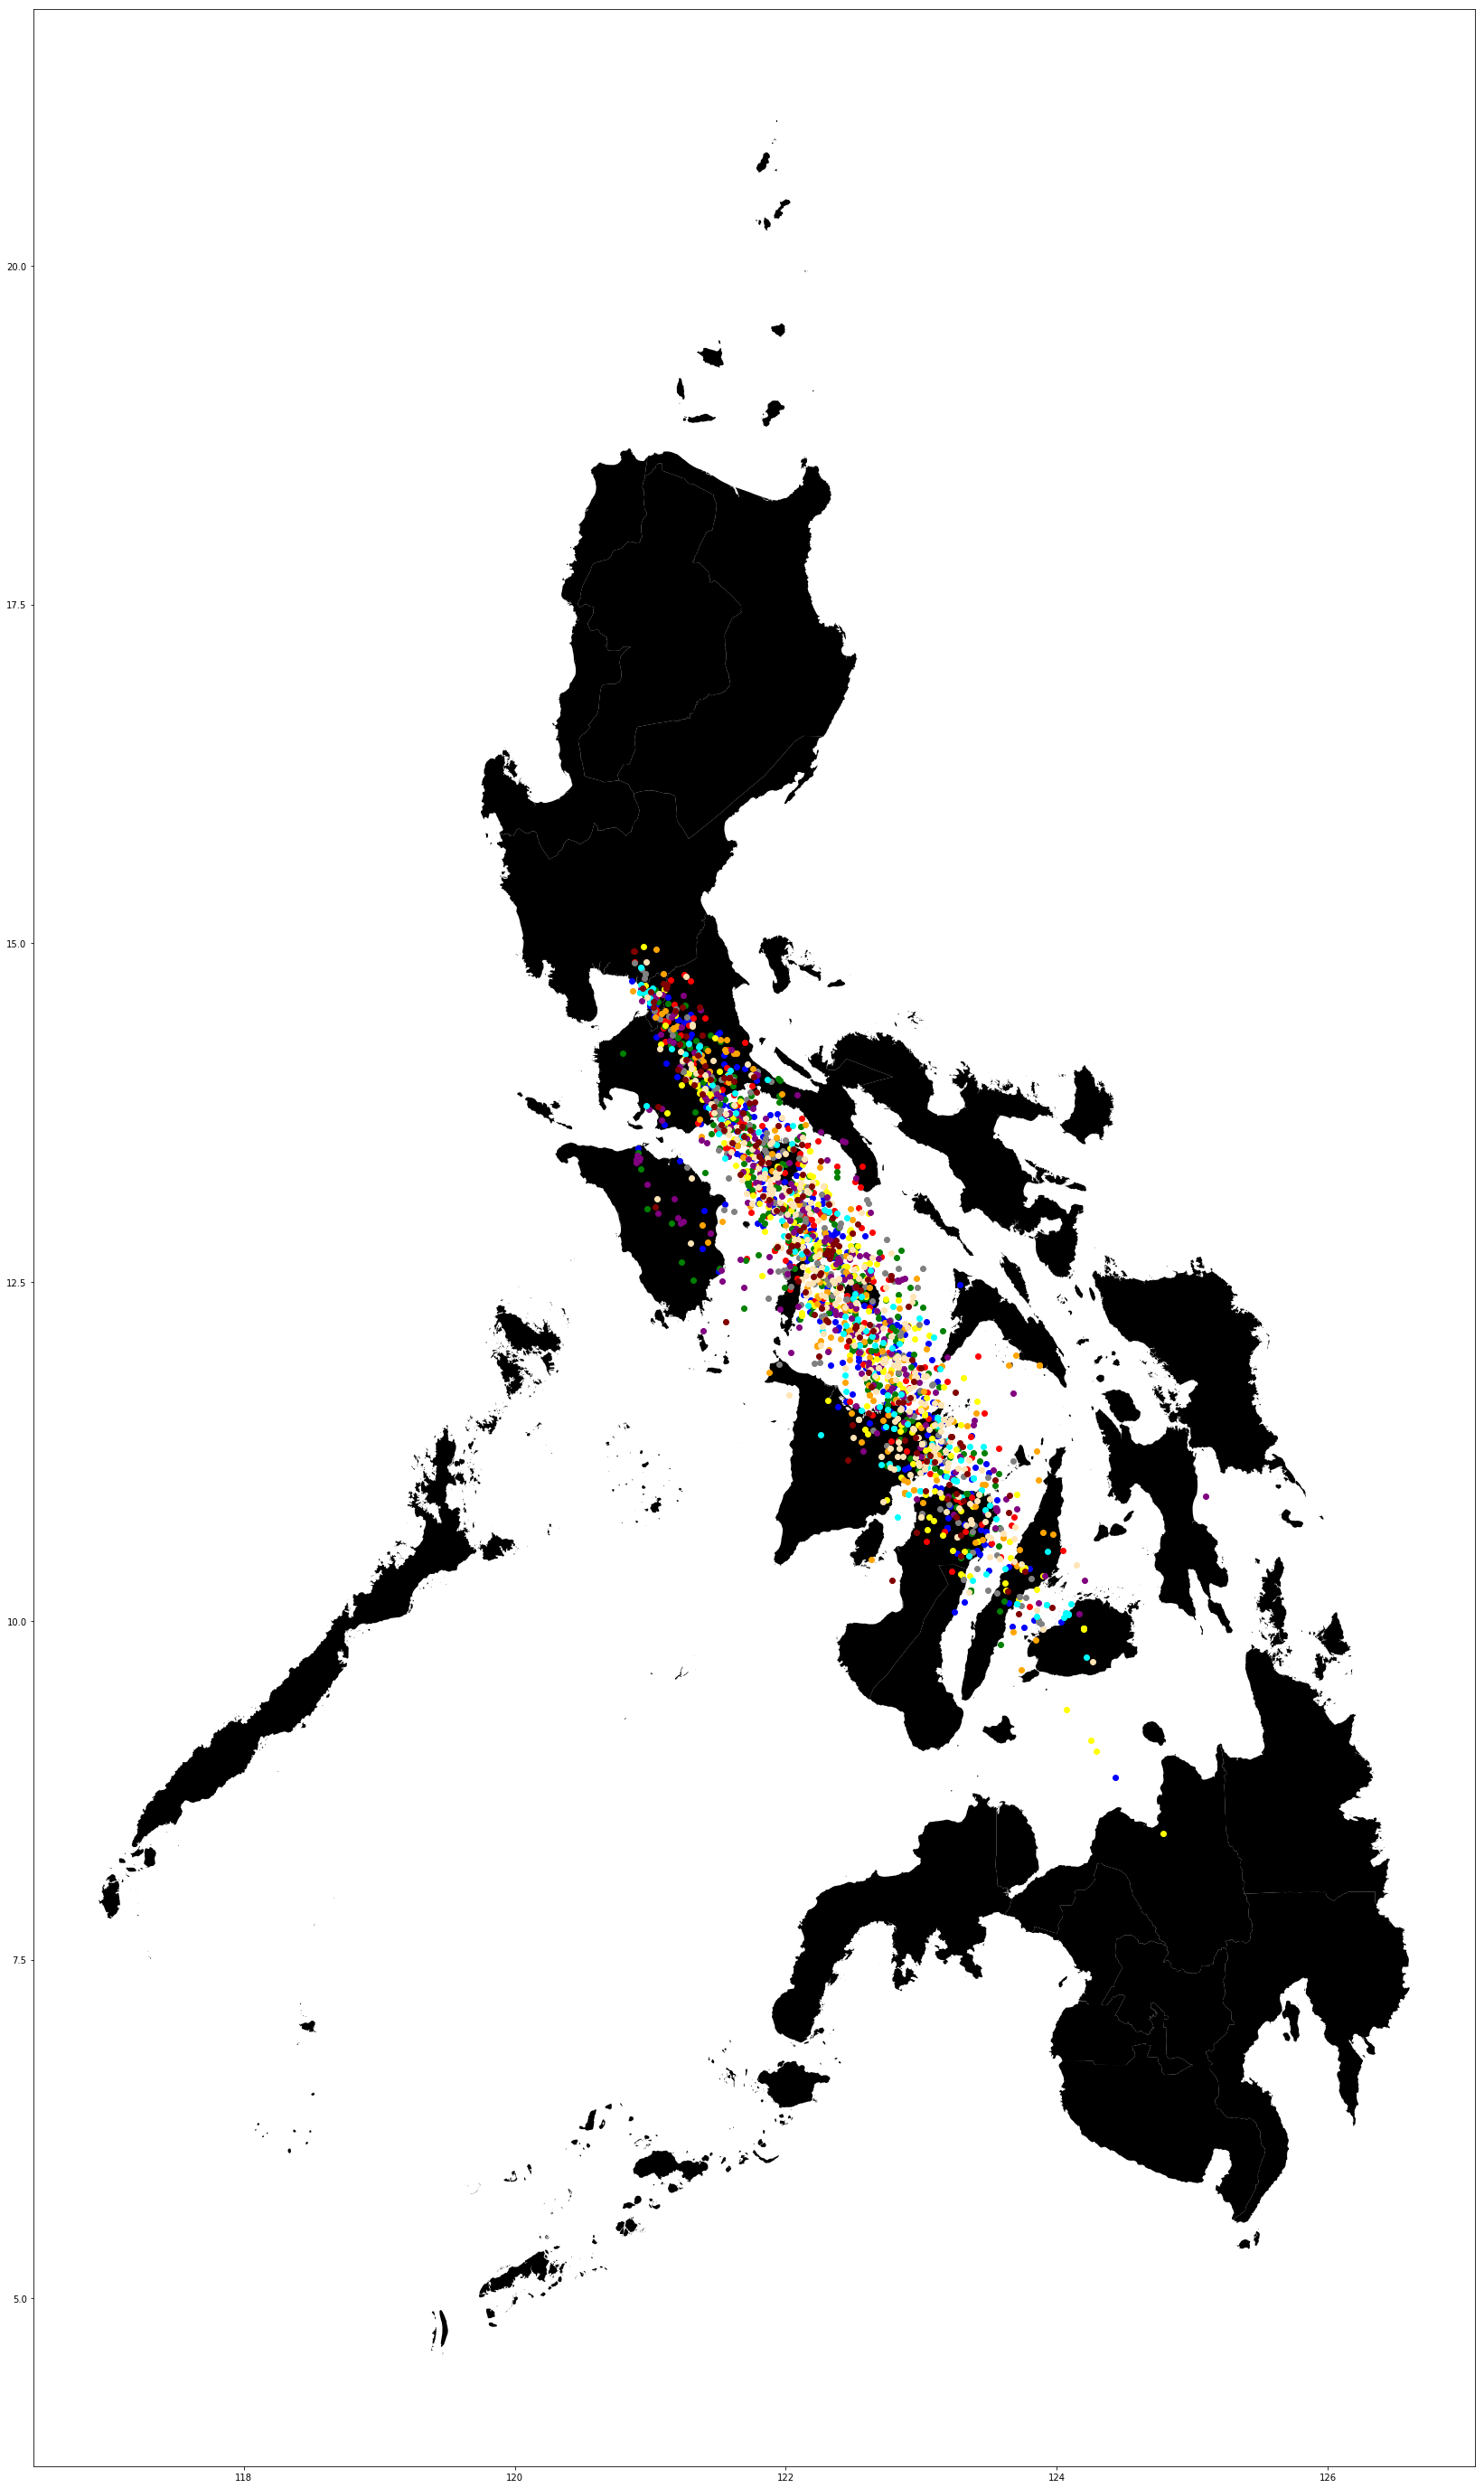
\includegraphics[width=\textwidth, height=\textheight,keepaspectratio]{Method1ApproxMap.png}
    \caption{LDA-LSA Double Filter Plot of Approximated Tweets}
    \label{fig:my_label2}
\end{figure}

\begin{figure}
    \centering
    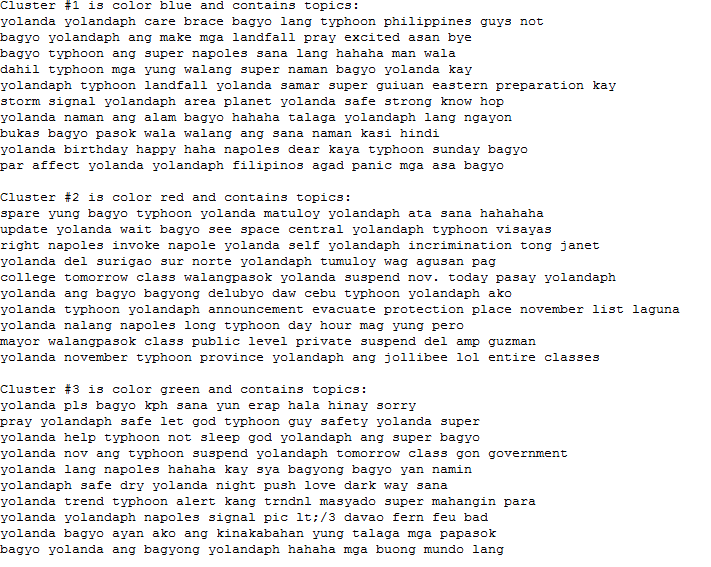
\includegraphics[width=\textwidth, height=\textheight,keepaspectratio]{Method1Cluster1.PNG}
    \caption{LDA-LSA Double Filter Clusters 1-3}
    \label{fig:my_label3}
\end{figure}


\begin{figure}
    \centering
    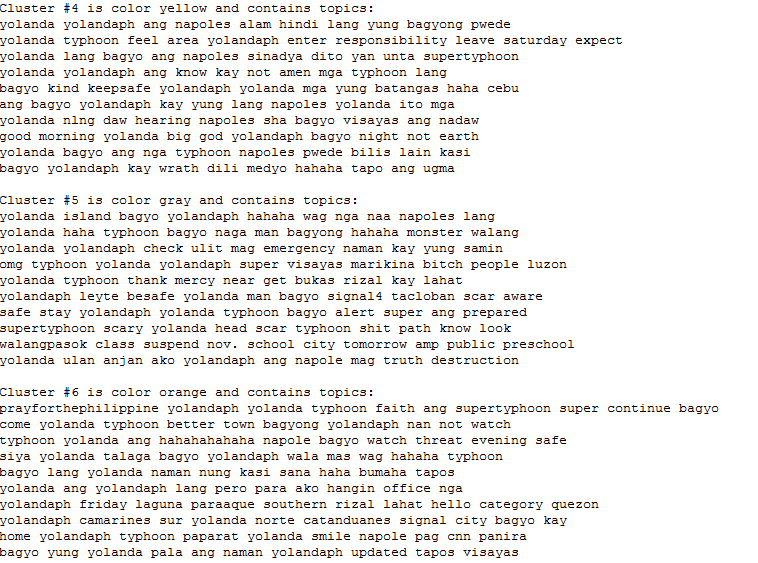
\includegraphics[width=\textwidth, height=\textheight,keepaspectratio]{Method1Cluster2.PNG}
    \caption{LDA-LSA Double Filter Clusters 4-6}
    \label{fig:my_label4}
\end{figure}

\begin{figure}
    \centering
    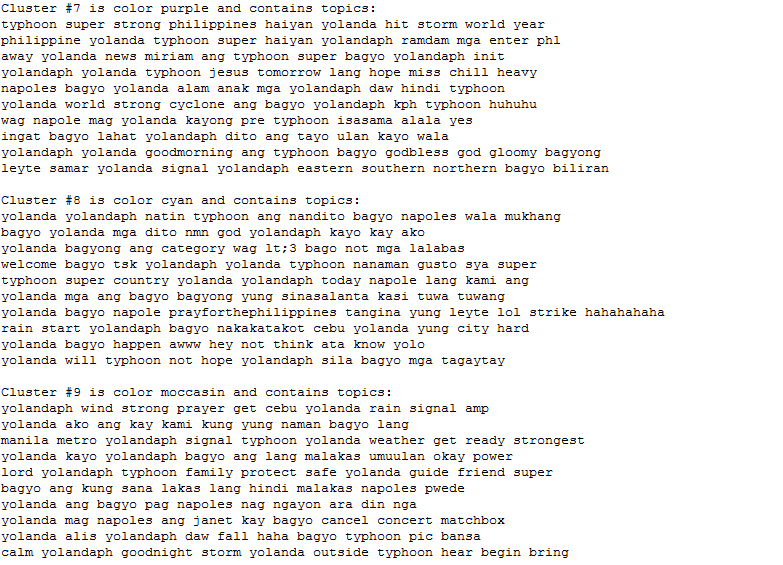
\includegraphics[width=\textwidth, height=\textheight,keepaspectratio]{Method1Cluster3.PNG}
    \caption{LDA-LSA Double Filter Clusters 7-9}
    \label{fig:my_label5}
\end{figure}

\begin{figure}
    \centering
    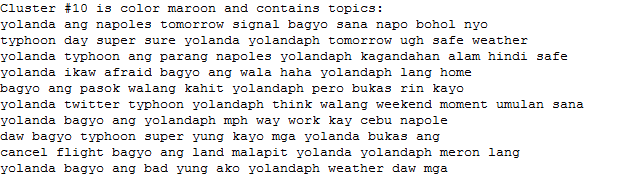
\includegraphics[width=\textwidth, height=\textheight,keepaspectratio]{Method1Cluster4.PNG}
    \caption{LDA-LSA Double Filter Cluster 10}
    \label{fig:my_label6}
\end{figure}

\begin{figure}
    \centering
    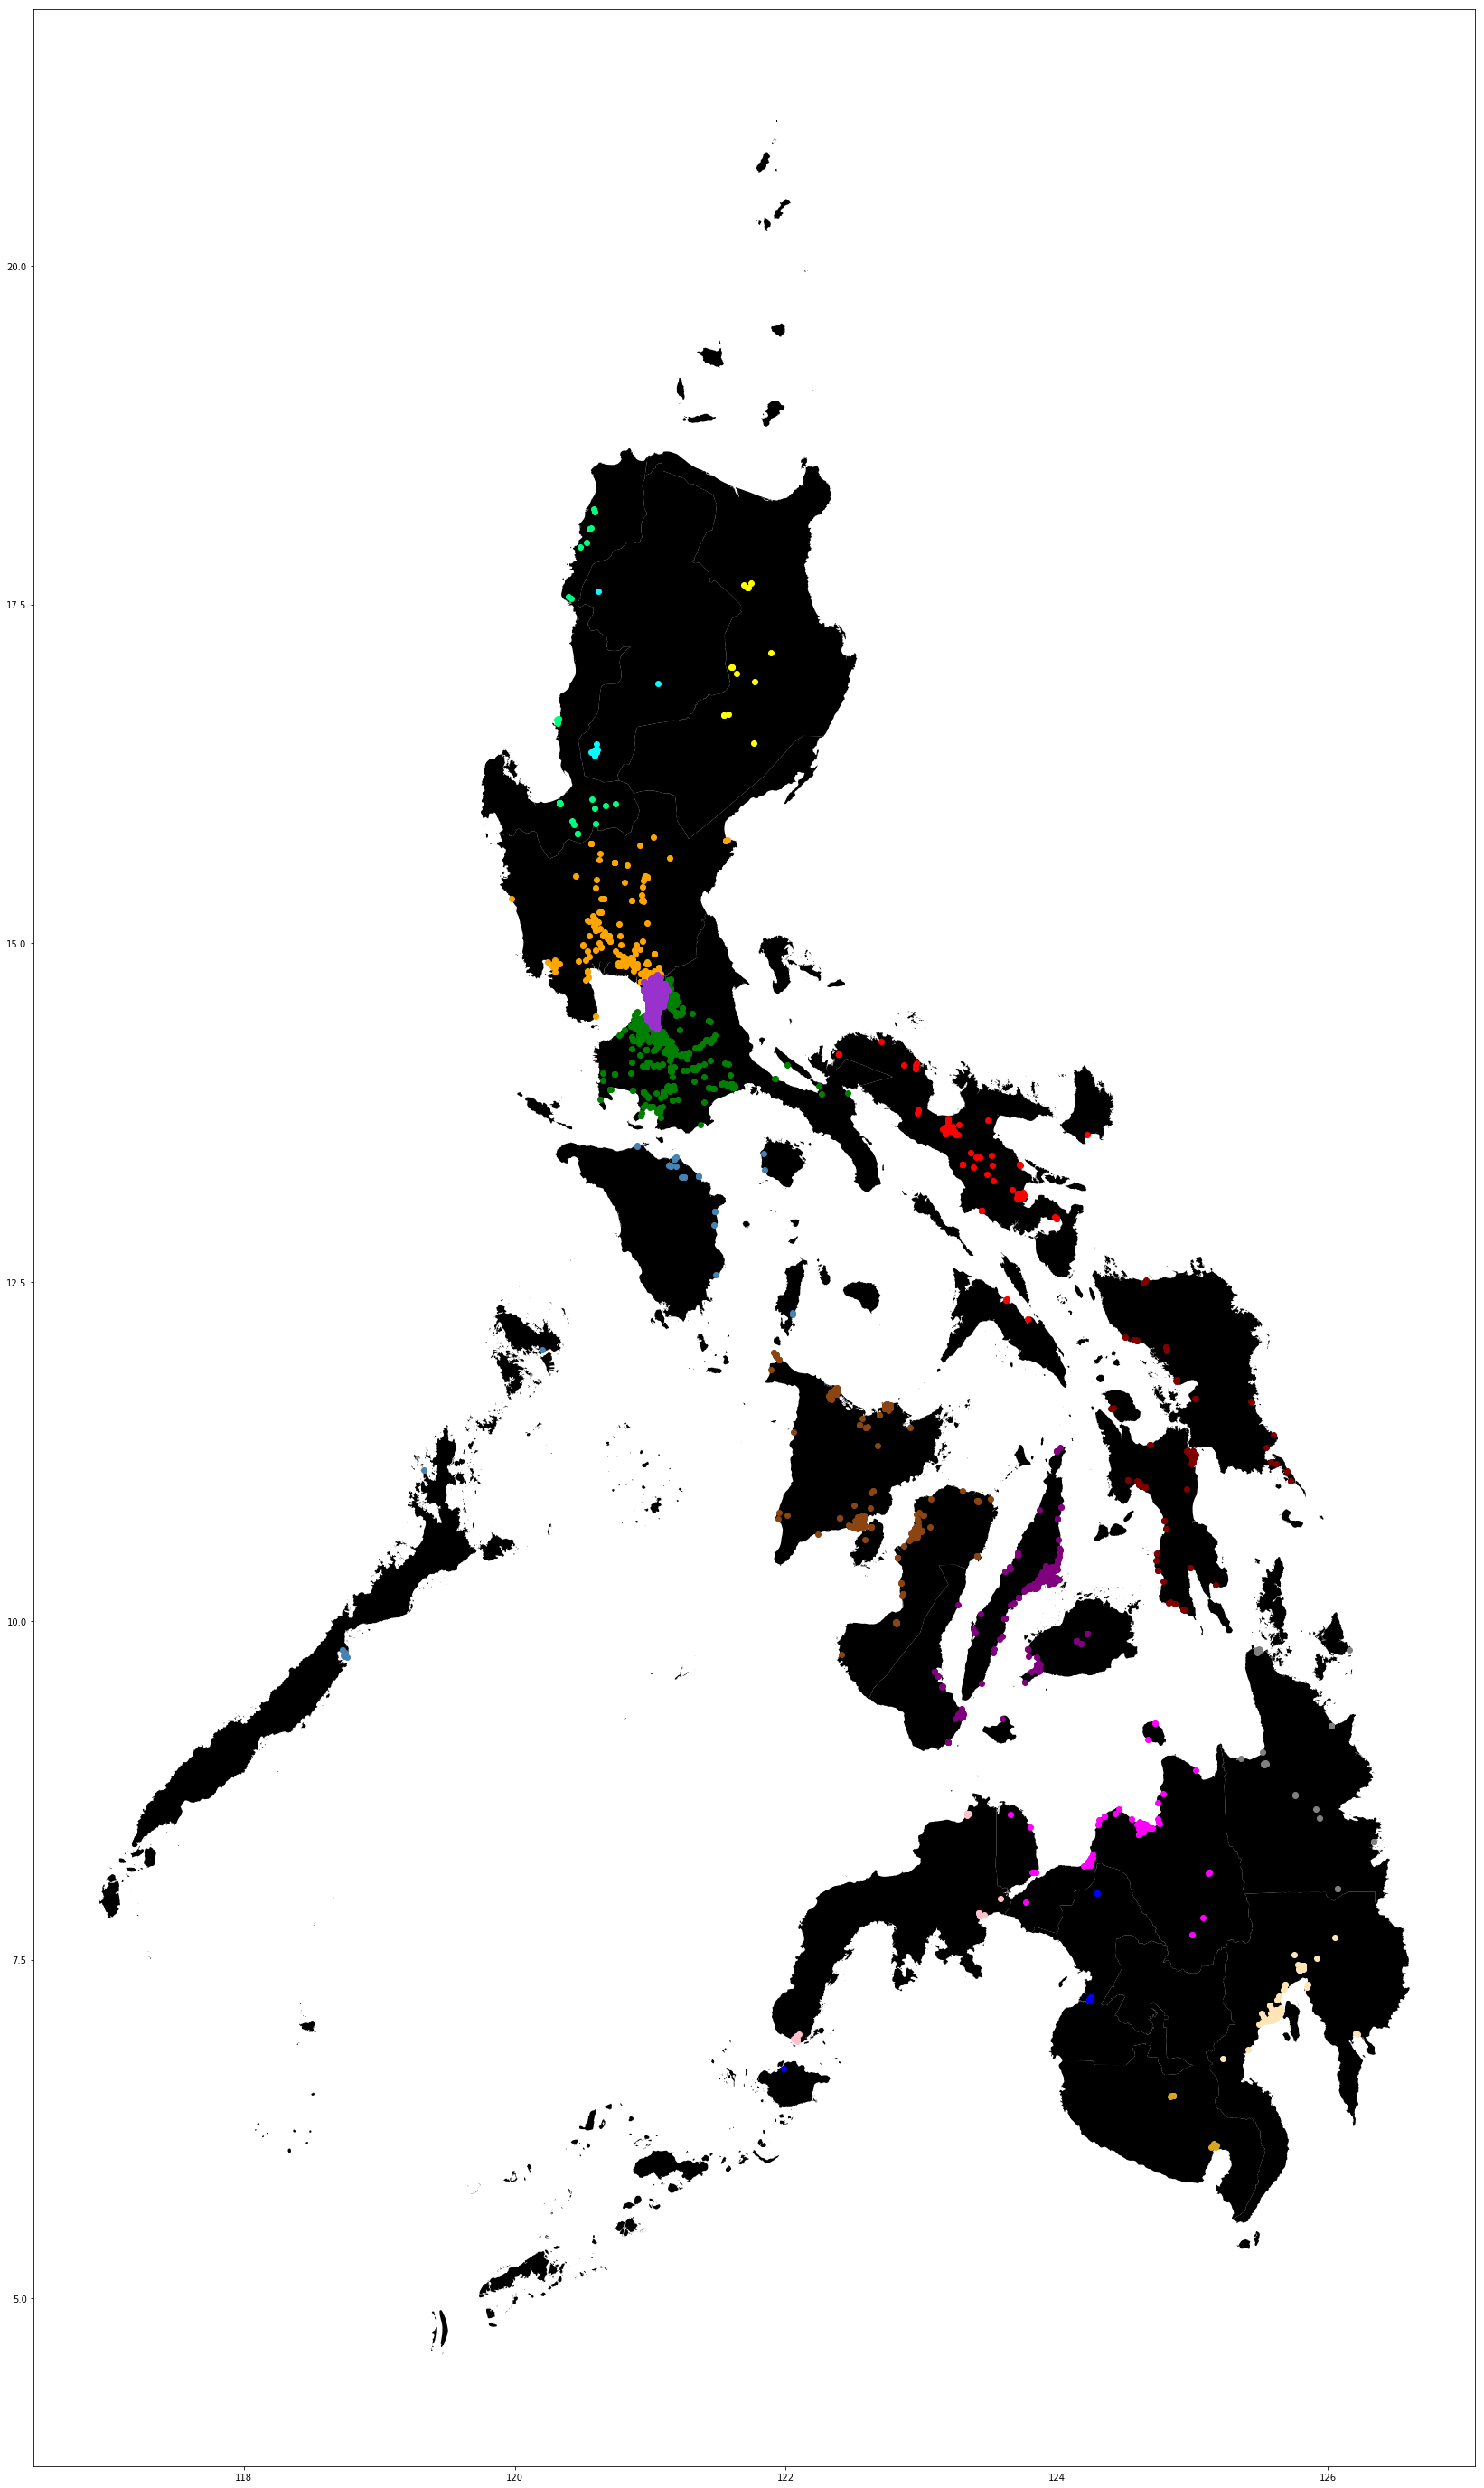
\includegraphics[width=\textwidth, height=\textheight,keepaspectratio]{Method2OrigMap.png}
    \caption{Dynamic Dictionaries Per Region Plot of Original Tweets}
    \label{fig:my_label7}
\end{figure}

\begin{figure}
    \centering
    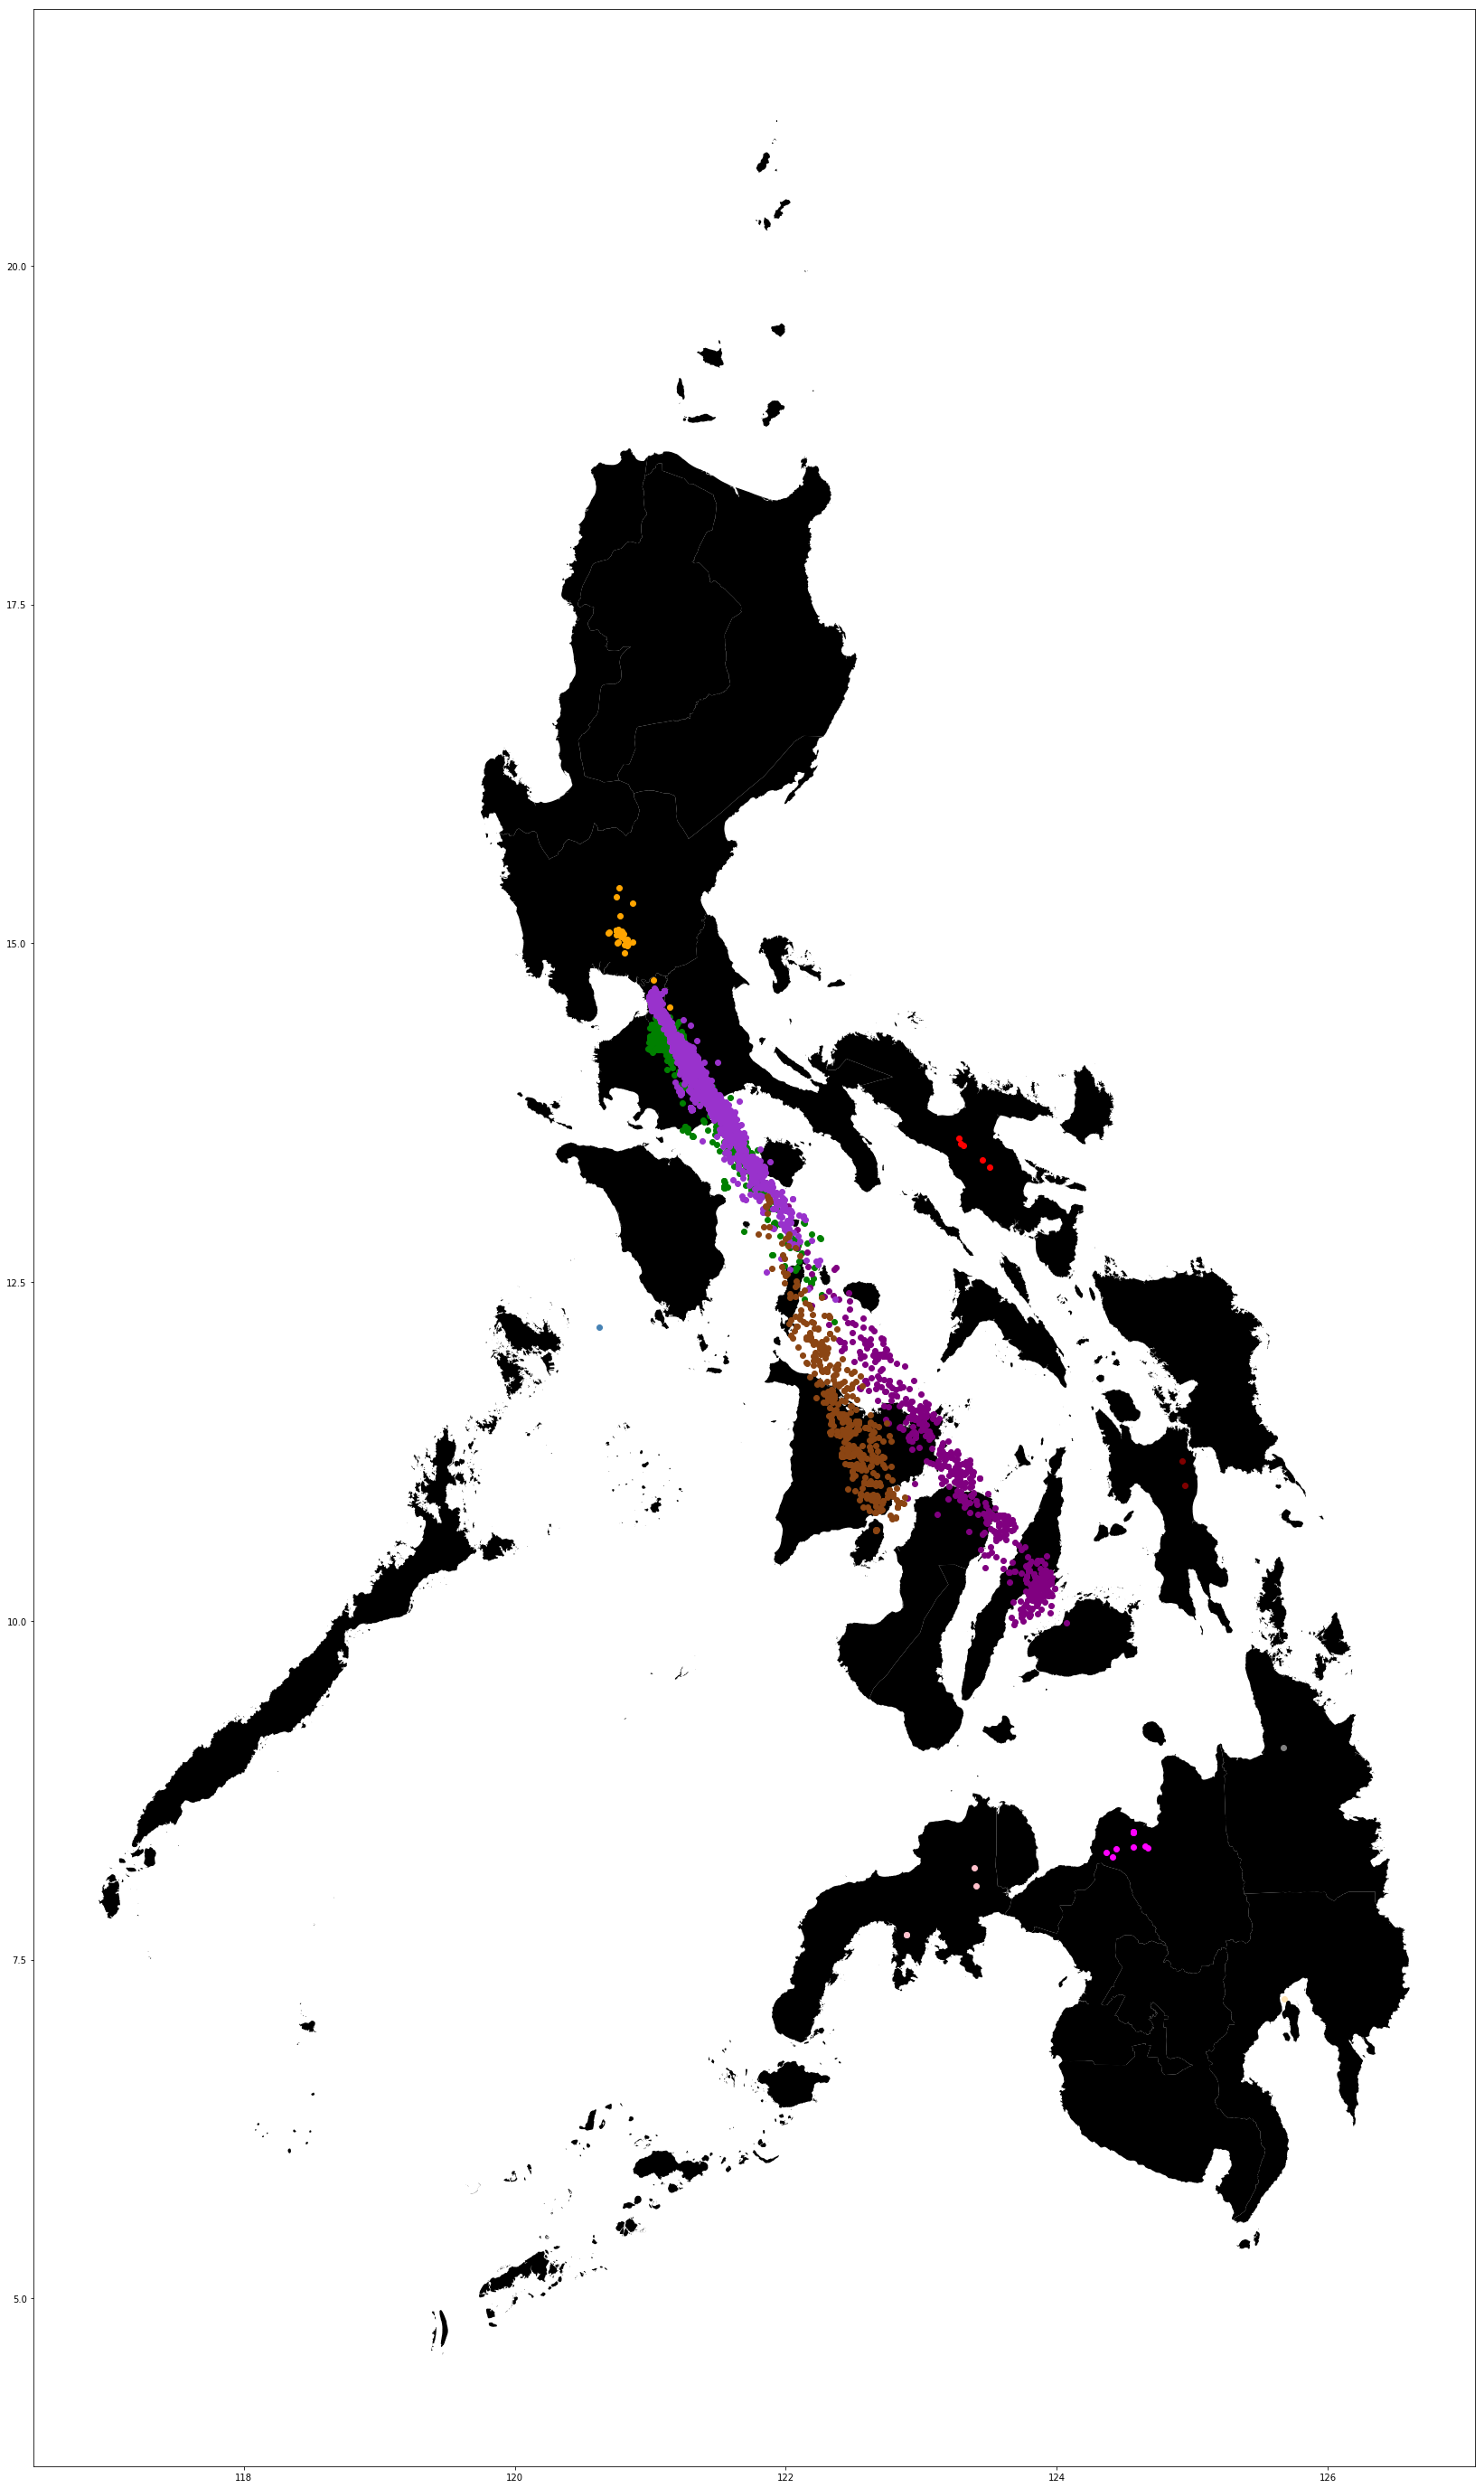
\includegraphics[width=\textwidth, height=\textheight,keepaspectratio]{Method2ApproxMap.png}
    \caption{Dynamic Dictionaries Per Region Plot of Approximated Tweets}
    \label{fig:my_label8}
\end{figure}

\begin{figure}
    \centering
    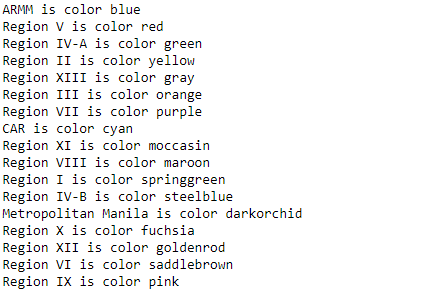
\includegraphics[width=\textwidth, height=\textheight,keepaspectratio]{Method2Cluster.PNG}
    \caption{Dynamic Dictionaries Per Region Clusters}
    \label{fig:my_label9}
\end{figure}

\subsection{LDA-LSA Double Filter Visualized Results}
Figure \ref{fig:my_label1} to \ref{fig:my_label6} shows the plots and cluster legend for the results of the first methodology. Figure \ref{fig:my_label1} shows that the original tweets that were clustered into the same topics were not necessarily within close geographic proximity among each other. In the case of some clusters, there were tweets that belonged in different parts of the Philippines. For example, there were tweets in Luzon and in Mindanao that were classified to the same cluster of topics. 

Figure \ref{fig:my_label2} shows the plot for the first methodology's geolocated tweets. As seen in the figure, the tweets belonging in the same cluster are more geographically clumped up together in general. It may be noted that the majority of the tweets were approximated to be located near the Visayas region and south of the NCR. It is also apparent that there are groups of tweets that were geolocated in invalid locations such as bodies of water. 

Figures \ref{fig:my_label3} to \ref{fig:my_label6} serve as the legend of clusters for Figures \ref{fig:my_label1} and \ref{fig:my_label2}. There were ten clusters used for the LDA-LSA Double Filter methodology. Each cluster contains ten topics in string form with similar themes. The ten clusters used reflect the number of topics that were used to train the LDA model as discussed in the methodology section. The color for each cluster of topics are also specified. 

\subsection{Dynamic Dictionaries Per Region Visualized Results}
Figures \ref{fig:my_label7} to \ref{fig:my_label9} display the plots and cluster legend for the Dynamic Dictionaries Per Region methodology. Figure \ref{fig:my_label7} contains the plot of the original tweets from the dataset used in this study. It may be observed that all Philippine geographic regions contain at least one tweet in their vicinity, with a majority of them being located in Central Luzon. 

Figure \ref{fig:my_label8} is the plot of the geolocated tweets from the Dynamic Dictionaries Per Region methodology algorithm. There are some Philippine geographic regions shown in Figure \ref{fig:my_label8} that do not contain any tweets unlike in Figure \ref{fig:my_label7}. It is also worth noting that there were groups of tweets that were geolocated in bodies of water similar to the case of the LDA-LSA Double Filter methodology. Lastly, Figure \ref{fig:my_label9} shows the legend of clusters for the Dynamic Dictionaries Per Region methdology.

All plots and figures were created via Python scripts. Any program that has Python support may recreate these plots accordingly. 

\section{Insights}
The results of both methodologies provide several insights. It appears that the first methodology (LDA-LSA Double Filter) outperformed the second (Dynamic Dictionaries Per Region) in all three metrics used to measure the accuracy of the results of both.

The closer to zero the Mean Absolute Error of a dataset is compared to another, the better. Again, a value of 0 indicates that the values of a test dataset completely matches that of the values of a given target dataset. The Mean Absolute Error value of the first methodology is lower by 0.3 compared to the second. This means that the approximated coordinates from the first methodology are closer to the actual coordinates in the dataset than the ones from the second.

The Haversine Formula and Vincenty Formula results show a similar trend. The first methodology's scores are significantly better than the second's for both metrics. This indicates that the approximated coordinates from the first methodology are nearer to their actual coordinates from dataset in terms of kilometers. This means that given these results, it is more effective to approximate a given disaster-related tweet according to the topic it belongs to than its geographic region. 

A possible reason as to why the second methodology yielded worse results is because there are some Philippine regions that cover relative large geographic areas. This means that it is possible that the approximated latitude and longitude coordinates of a given tweet belongs in the same region as its original coordinates, but not necessarily in the same vicinity. Some areas within certain Philippine regions are separated by tens or even hundreds of kilometers. This may contribute to high distance disparity between the actual and approximated values. This is perhaps the main drawback of classifying tweets per region. 

Another possible reason as to why the first methodology outperformed the second is the structure of the dataset that was used in this study. It was found that over sixty percent of the tweets in the dataset belonged in the NCR and that some regions contained anywhere from nine to twenty-five tweets only. This may cause the execution of the second methodology to perform worse because the models representative of all geographic regions are not equally refined/trained. There are some models that are more refined than others since the number of tweets are not equally distributed across all available regions. This conversely means that some models are poorly trained because there are only several tweets from that region as far as the dataset used is concerned. The differences in refinement of the geographic models may cause the models to classify a given query tweet to the incorrect region because it is more likely that the more refined models will be selected by the algorithm described in the previous sections. The richer models have more depth in terms of stored information and thus are more capable of processing and identifying incoming query tweets as part of the geographic region they represent. It is highly likely that there are many cases where, for example, a tweet originally from the ARMM region may be recognized and classified as a tweet from the NCR since the model representative of the latter region is much better trained. This kind of scenario becomes increasingly likely to happen as the algorithm executes because the models refresh periodically after processing a certain number of tweets. The better trained models will be continuously further trained and refined as they process more tweets.

These results however do not discount the fact that both methodologies still performed better than previous studies did as far as the Typhoon Yolanda tweets are concerned. An over 200 kilometer distance is still large, but this is a significant improvement from the findings of the previous studies discussed in the theoretical background section of this paper. The said previous studies had results of over 300 kilometers of distance for the approximated coordinates. Both methodologies had below 300 kilometers, which is a slight improvement. But again, the results indicate that while both methodologies are possible steps towards the right direction, the first methodology appears to be the more optimal approach for this dataset. It is also worth noting that the results of both methodologies showed that there were still quite a number of tweets that were geolocated in invalid locations such as bodies of water. Again, this is reflective of the fact that the Philippines is an archipelago, and that both methodologies may still be improved tremendously. 
%\input{04_results_pub}
%\input{04_results_unpub}
\chapter{CONCLUSIONS}
The results of this study show improvements from the results of previous studies regarding the location approximation of disaster-related tweets using Latent Semantic Analysis. However, the structure of the dataset of tweets used may have influenced just exactly how big these improvements actually are. Nevertheless, the implementation and execution of both methodologies showed that there are different approaches that may be used alongside Latent Semantic Analysis in the context of location approximation. 

It was discussed in the introduction section of this paper that the main question this study aimed to address is concerned with exploring different methods for a more fine-tuned geolocation approximation algorithm. The results presented in the previous section offer an answer to this said question. Perhaps generating topics from the available tweets and classifying tweets according to specific geographic regions may be a possible starting point for further fine-tuning of LSA based geolocation. The results of both methodologies also offer possible answers to the sub-questions mentioned in the introduction section.

\section{Modifications Of LSA Based Location Approximation}
The first sub-question mentioned in the introduction section of this study dealt with what possible modifications to the LSA algorithm may be made to produce a more fine-tuned approach to the geolocation of disaster-related tweets. Both methodologies address this particular sub-question.

The first methodology (LDA-LSA Double Filter) of this study was concerned with first using Latent Dirichlet Allocation to extract underlying themes in the dataset of tweets and performing Latent Semantic Analysis based on said themes. Generating possible topics from a set of tweets and processing each tweet according to the topic/s it contributes to makes for a more structured approach. The tweets were essentially grouped according to topics so that LSA will be performed using the topics as reference as opposed to iterating over the entire dataset for each incoming query. Iterating over the generated topics means that it is more likely that the tweets that will be included in the geolocation of a given query will be related to the said query in terms of meaning. Analyzing a particular tweet relative to a set of other tweets that pertain to a common topic follows the presupposition of this study that semantically similar tweets most likely come from the same general location. If a disaster event takes place in a given area then disaster-related tweets from citizens near that said area will more or less have a specific common subject. This was the main principle behind this specific modification to the LSA approach.

The second methodology (Dynamic Dictionaries Per Region) on the other hand builded on the recommendations of previous Latent Semantic Analysis based studies. The particular recommendation essentially stated that narrowing the area of where to consider tweets that will be included in the geolocation of a given query may yield more favorable results. This was done by training LSA models representative of each Philippine geographic region. Identifying which region a query tweet most likely belongs to makes iterating over the entire dataset unnecessary. Instead only the tweets that belong in the selected region are considered and used in analysis. Using LSA on its own to analyze the tweets in the dataset would entail considering tweets from Luzon, Visayas, and Mindanao to approximate the coordinates of a given query. This may be problematic in some cases since the Philippines is an archipelago and the distance between the three island groups of the country is vast. As an example, suppose tweets from Luzon and Mindanao are used to approximate the location of a given query tweet. The resulting value would be skewed because the convex hull that will be constructed to approximate the query's coordinates covers a very large area. Narrowing the area enclosed by the convex hull of tweets lowers the likelihood of this potential occurrence. 

\section{Visualization of Results and Availability For External Programs}
All LSA and LDA models were implemented and trained in Python. The trained models may be imported to any Python program with access to the Python library Gensim. Once imported, the models may be used for queries or even retrained within the program. The Python library Geopandas is also required to replicate the steps of the second methodology that is concerned with classifying a given tweet to a particular Philippine geographic region. 

As of now it is unknown if there are any other programming languages or platforms that may access the trained models completely. The official documentation for the Gensim and Geopandas libraries are only defined for Python.

As mentioned in the results section, the visualizations of the results of both methodologies of this study were created in Python as well. The Python libraries Geopandas and Matplotlib were used to create all the corresponding visualizations and figures. Any program that has access to these two Python libraries will be able to recreate the plots shown in the results section. 

%Upon presenting your results, the conclusion is where you will now %tie up these results with the original intent of the study, as %indicated by the research questions given in the Introduction. It is %in this section where you will also discuss any difficulties or %issues encountered during the study, as well as your recommended %method for addressing these problems.

%The general way to organize your conclusion is to present each %research sub-question as a subsection, and thoroughly answer each of %them by interpreting your results with respect to the question. With %these answered, you may then tie up all of your findings in each %subsection to answer your main research question, providing any %needed additional information or explanation. Last on the list would %be your unsolved issues and difficulties, presenting them as avenues %to motivate continued work on your chosen topic.

\chapter{RECOMMENDATIONS}
The results of this study indicate that there is still more room for improvement with regards to Latent Semantic Analysis based geolocation. It was mentioned in the results section that the average distance   the approximated and actual location of the processed tweets is over two hundred kilometers for both methodologies. Two hundred kilometers is still quite a large gap especially for disaster-related tweets. It is important that accurate disaster-related information be disseminated quickly and efficiently in order to help respondents act accordingly. That being said the following sections will discuss several possible modifications to the methodologies of this study that may potentially fine-tune them further.

\section{LDA-LSA Double Filter}
A possible modification to the first methodology is concerned with choosing a different number of topics for training all models. One hundred and two hundred topics were specified for the Latent Dirichlet Allocation models and Latent Semantic Analysis models respectively. The main reason for choosing these numbers of topics for the models is to follow Python conventions. Two hundred topics is the recommended number for training Python models in general as discussed in the official Gensim documentation. This number was lessened for the LDA models based on the observation that there is usually a limited number of disaster-related topics during times of disaster. Disaster-related tweets also usually do not contain many sub-topics. 

It is possible that there is a more optimal number of topics that may be used to train LDA and LSA models which will yield more accurate results. It may be argued that training models with less topics, especially the LDA model, is reasonable behind the observation that disaster topics tend to be specific and usually do not have many branching sub-topics. In this case the algorithm will have less iterations which may improve its overall run    time and allow more queries to be processed. Training the models with less topics will also lessen the likelihood that duplicate or synonymous topics
will be generated. This may help polish the algorithm further as less redundant topics will be considered for each query.

\section{Dynamic Dictionaries Per Region}
The structure of the dataset used in this study may have impacted the overall performance of the second methodology as mentioned in
the results section. The models representative of the Philippine geographic regions are not equally refined as a result of an unequal distribution of tweets from each region. This results in cases where the distance between the actual and approximated 
location of a given query is considerably large. Incorrectly identifying the region of a tweet causes this problem since the Philippines is an archipelago and each region covers a vast area. The distance between two Philippine regions may span from tens to hundreds of kilometers.

A possible way to address this scenario is to train models representative of smaller spaces such as cities/provinces and districts. Doing so may lessen the distance between the actual and approximated location for some queries. Classifying a query to an incorrect area may not always drastically influence its approximated coordinates because it is possible that the actual location of the said query is not that far from the approximated one. However it is worth noting that training more models would result in more poorly refined models since the distribution of tweets in the dataset is not equally distributed around the Philippines. There may be models that will not contain tweets at all, and some may contain only a handful. But this may be the overall more optimal approach especially when dealing with bigger data as more areas will be represented by a particular LSA model. This allows queries to be processed with more specific information as the algorithm will consider more geographic spaces.

%% \section{Thesis Formatting Guidelines}

% This thesis template in Word document format was created to ensure that you will spend more time generating content for your paper and less time stressing about formatting issues. To ensure, however, that your document is truly formatted according to specifications, here are some formatting guidelines which you may use to evaluate your own paper’s formatting.

% \begin{enumerate}
% \item There should be NO PAGE NUMBERS on the first page of every chapter/section..
% \item Tables must have NO VERTICAL LINES, as well as NO INNER HORIZONTAL LINES after the table headers.
% \item Figures and tables are numbered ACCORDING TO CHAPTER NUMBER (e.g. Table 3.1 must be located in Chapter 3, and Figure B.2 is in Appendix B).
% \item The sequence of front matter must be as follows:
%     \begin{enumerate}
%     \item Title Page, in the correct formatting (e.g. Titles must be written in an inverted triangle, in ALL CAPS and boldface)
%     \item Abstract
% 	\item Table of Contents
% 	\item List of Figures
% 	\item List of Tables
% 	\end{enumerate}
% \item Upon binding, the front cover must contain the EXACT CONTENT AND FORMAT as that of your thesis’ title page.
% \end{enumerate}

\chapter{Sample GeoJSON Tweet Output}

\begin{figure}[hbt!]
    %\centering
    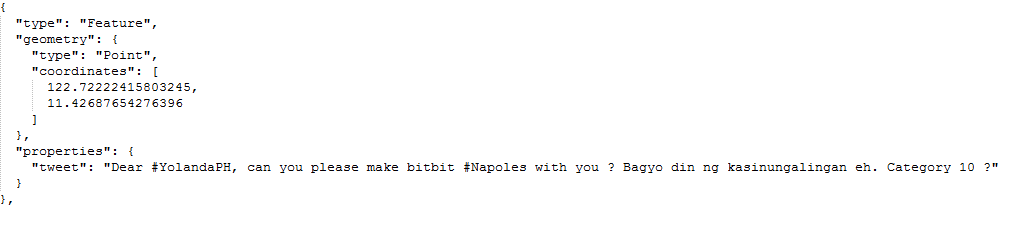
\includegraphics[width=\textwidth, height=\textheight,keepaspectratio]{GeoQuery.PNG}
    \caption{Sample Tweet GeoJSON Data.}
    %\label{fig:my_label}
\end{figure}

% BIBLIOGRAPHY
%\bibliographystyle{abbrv}
\bibliographystyle{plain}
\bibliography{sigproc}
%\input{09_references}
% \BackMatter

%\bibliography{Proposal_Manuscript}
\addappheadtotoc
\begin{appendices}
%\chapter{Geolocation Query Visualization}
% \section{Introduction to the Appendices}

% The Appendices is where you are enabled to present any additional or supplementary information relevant to your study, yet do not require highlighting within the actual paper, either because of its trivial nature or volume. These may in the form of figures, tables, or additional text detailing specific aspects about or related to the study.

% \section{Sample Questions for Different Studies}
% The following table presents three sample studies, as well as the guide questions that may help direct the discussion in each section of the paper. You may use this as another reference in writing your paper.

%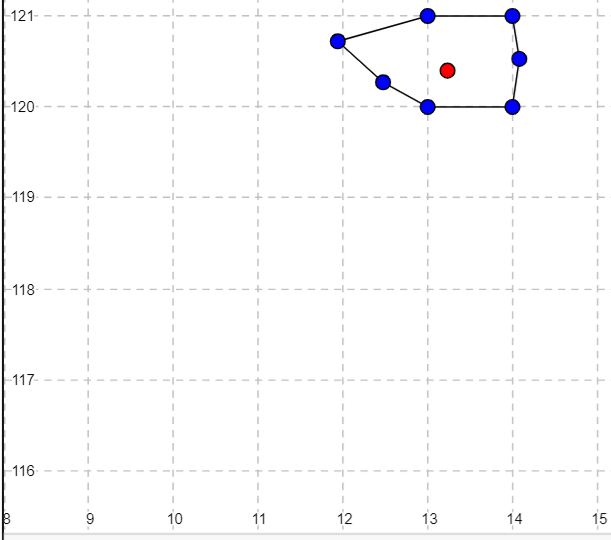
\includegraphics[width=\textwidth]{SampleThesisQuery.PNG}

\chapter{Geolocation Query Visualization}



\begin{figure}[hbt!]
    %\centering
    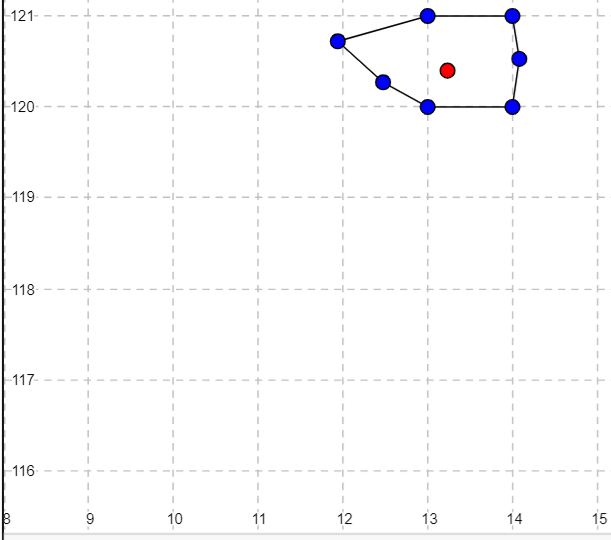
\includegraphics[width=\textwidth, height=\textheight,keepaspectratio]{SampleThesisQuery.PNG}
    \caption{Sample Query Visualization. Red point indicates approximated tweet. Blue points indicate already-geolocated tweets.}
    %\label{fig:my_label}
\end{figure}


%\chapter{THESIS FORMATTING GUIDELINES}
% \section{Thesis Formatting Guidelines}

% This thesis template in Word document format was created to ensure that you will spend more time generating content for your paper and less time stressing about formatting issues. To ensure, however, that your document is truly formatted according to specifications, here are some formatting guidelines which you may use to evaluate your own paper’s formatting.

% \begin{enumerate}
% \item There should be NO PAGE NUMBERS on the first page of every chapter/section..
% \item Tables must have NO VERTICAL LINES, as well as NO INNER HORIZONTAL LINES after the table headers.
% \item Figures and tables are numbered ACCORDING TO CHAPTER NUMBER (e.g. Table 3.1 must be located in Chapter 3, and Figure B.2 is in Appendix B).
% \item The sequence of front matter must be as follows:
%     \begin{enumerate}
%     \item Title Page, in the correct formatting (e.g. Titles must be written in an inverted triangle, in ALL CAPS and boldface)
%     \item Abstract
% 	\item Table of Contents
% 	\item List of Figures
% 	\item List of Tables
% 	\end{enumerate}
% \item Upon binding, the front cover must contain the EXACT CONTENT AND FORMAT as that of your thesis’ title page.
% \end{enumerate}

\chapter{Sample GeoJSON Tweet Output}

\begin{figure}[hbt!]
    %\centering
    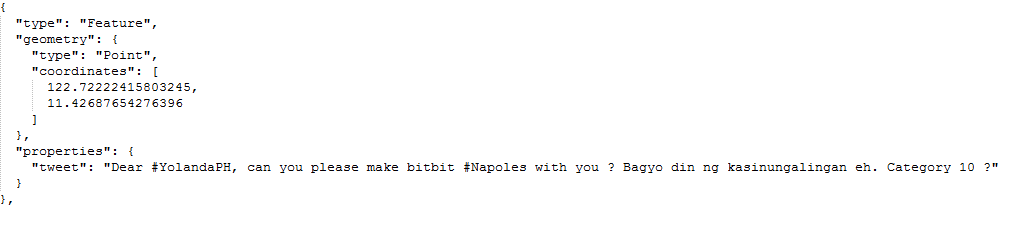
\includegraphics[width=\textwidth, height=\textheight,keepaspectratio]{GeoQuery.PNG}
    \caption{Sample Tweet GeoJSON Data.}
    %\label{fig:my_label}
\end{figure}

\chapter{Methodology 1 Algorithm Tweet Query}

\begin{figure}[hbt!]
    %\centering
    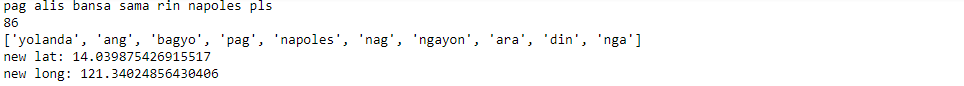
\includegraphics[width=\textwidth, height=\textheight,keepaspectratio]{Method1Query.PNG}
    \caption{Second line indicates topic number. Following line shows top contributing words of said topic.}
    %\label{fig:my_label}
\end{figure}
\chapter{Methodology 2 Algorithm Tweet Query}

\begin{figure}[hbt!]
    %\centering
    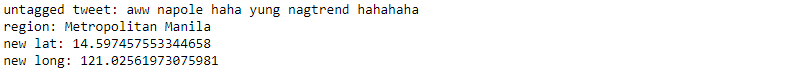
\includegraphics[width=\textwidth, height=\textheight,keepaspectratio]{Method2Query.PNG}
    %\caption{}
    %\label{fig:my_label}
\end{figure}

\end{appendices}


\end{document}